\documentclass[11pt,a4paper]{article}

% Inclusión de paquetes y configuración general
% ==============================================================================
% PAQUETES DE LATEX PARA DOCUMENTACIÓN TÉCNICA FORMAL ERS SYSELL
% ==============================================================================

\usepackage[utf8]{inputenc}
\usepackage[T1]{fontenc}
\usepackage[spanish,es-tabla,es-nodecimaldot]{babel}

% Geometría y márgenes
\usepackage[top=2.5cm, bottom=2.5cm, left=2.5cm, right=2.5cm, headheight=16pt]{geometry}

% Tipografía y microtipografía
\usepackage{lmodern}
\usepackage{microtype}
\usepackage{amsmath, amssymb, amsfonts}

% Tablas avanzadas
\usepackage{booktabs}
\usepackage{tabularx}
\usepackage{colortbl}
\usepackage{array}
\usepackage{longtable}

% Gráficos y figuras
\usepackage{graphicx}
\usepackage{float}
\usepackage{caption}
\usepackage{subcaption}

% Colores
\usepackage[x11names,dvipsnames,table]{xcolor}

% Cajas de texto y requisitos destacados
\usepackage{tcolorbox}

% Diagramación vectorial TikZ
\usepackage{tikz}
\usetikzlibrary{shapes.geometric, arrows.meta, positioning, calc, backgrounds, fit, matrix}

% Encabezados y pies de página
\usepackage{fancyhdr}

% Títulos de secciones personalizados
\usepackage{titlesec}

% Listas personalizadas
\usepackage{enumitem}

% Listados de código fuente
\usepackage{listings}

% Hipervínculos e índice interactivo
\usepackage{hyperref}

% Símbolos adicionales
\usepackage{pifont}


% Inclusión de estilos corporativos y definiciones
% ==============================================================================
% ESTILOS, COLORES Y AMBIENTES PERSONALIZADOS PARA SYSELL
% ==============================================================================

% Paleta de colores institucionales y de ingeniería
\definecolor{PrimaryBlue}{RGB}{14, 43, 92}      % Azul institucional profundo
\definecolor{SecondaryBlue}{RGB}{30, 90, 160}   % Azul secundario
\definecolor{AccentTeal}{RGB}{0, 150, 136}      % Teal / Verde azulado
\definecolor{DarkSlate}{RGB}{44, 62, 80}        % Gris pizarra oscuro
\definecolor{LightSlate}{RGB}{244, 247, 250}    % Fondo claro para tablas
\definecolor{AlertRed}{RGB}{185, 28, 28}        % Rojo para advertencias / reglas
\definecolor{SuccessGreen}{RGB}{22, 101, 52}    % Verde éxito
\definecolor{BorderGray}{RGB}{203, 213, 225}    % Gris para bordes suaves
\definecolor{CodeBg}{RGB}{248, 250, 252}        % Fondo para código

% Configuración de Hyperref
\hypersetup{
    colorlinks=true,
    linkcolor=SecondaryBlue,
    citecolor=AccentTeal,
    urlcolor=SecondaryBlue,
    filecolor=DarkSlate,
    pdfauthor={Johan Mamani, Luis Condori, Aron Cachicatari, Giorgini Pacci},
    pdftitle={Especificación de Requisitos de Software y Arquitectura Web - SYSELL},
    pdfsubject={Ingeniería de Software I - UNJBG},
    pdfkeywords={ERS, IEEE 830, ISO 29148, ISO 25010, Clean Architecture, CQRS, React, Laravel, MySQL}
}

% Estilo de Encabezados y Pies de Página
\pagestyle{fancy}
\fancyhf{}
\fancyhead[L]{\small\scshape\color{DarkSlate} SYSELL --- Sistema Web de Gestión de Inventario y Ventas}
\fancyhead[R]{\small\color{SecondaryBlue}\textbf{IEEE 830 / ISO 29148}}
\fancyfoot[L]{\small\color{gray} UNJBG --- ESIS --- Ingeniería de Software I}
\fancyfoot[R]{\small\color{DarkSlate}\textbf{Página \thepage}}
\renewcommand{\headrulewidth}{0.8pt}
\renewcommand{\footrulewidth}{0.4pt}

% Configuración de títulos de secciones
\titleformat{\section}
  {\Large\bfseries\color{PrimaryBlue}}
  {\thesection}
  {1em}
  {}
  [{\color{BorderGray}\titlerule[0.8pt]}]

\titleformat{\subsection}
  {\large\bfseries\color{SecondaryBlue}}
  {\thesubsection}
  {0.8em}
  {}

\titleformat{\subsubsection}
  {\normalsize\bfseries\color{DarkSlate}}
  {\thesubsubsection}
  {0.6em}
  {}

% Ambientes tcolorbox estándar y compatibles
\newtcolorbox{reqbox}[3][]{
    colback=white,
    colframe=SecondaryBlue,
    coltitle=white,
    fonttitle=\bfseries\small,
    title={\textbf{#2:} #3},
    arc=3pt,
    boxrule=1pt,
    left=8pt, right=8pt, top=8pt, bottom=8pt,
    #1
}

\newtcolorbox{rnbox}[3][]{
    colback=white,
    colframe=AccentTeal,
    coltitle=white,
    fonttitle=\bfseries\small,
    title={\textbf{#2:} #3},
    arc=3pt,
    boxrule=1pt,
    left=8pt, right=8pt, top=8pt, bottom=8pt,
    #1
}

\newtcolorbox{hubox}[3][]{
    colback=LightSlate,
    colframe=DarkSlate,
    coltitle=white,
    fonttitle=\bfseries\small,
    title={\textbf{#2:} #3},
    arc=3pt,
    boxrule=1pt,
    left=8pt, right=8pt, top=8pt, bottom=8pt,
    #1
}

\newtcolorbox{infobox}[2][]{
    colback=LightSlate,
    colframe=SecondaryBlue,
    coltitle=PrimaryBlue,
    fonttitle=\bfseries,
    title={#2},
    arc=3pt,
    boxrule=1pt,
    left=8pt, right=8pt, top=8pt, bottom=8pt,
    #1
}

% Configuración de listings para código JSON, SQL, PHP, TypeScript
\lstset{
    backgroundcolor=\color{CodeBg},
    basicstyle=\ttfamily\footnotesize\color{DarkSlate},
    keywordstyle=\bfseries\color{SecondaryBlue},
    stringstyle=\color{AccentTeal},
    commentstyle=\itshape\color{gray},
    numbers=left,
    numberstyle=\tiny\color{gray},
    stepnumber=1,
    numbersep=8pt,
    frame=single,
    rulecolor=\color{BorderGray},
    breaklines=true,
    breakatwhitespace=true,
    showstringspaces=false,
    tabsize=2,
    captionpos=b
}


\begin{document}

% ------------------------------------------------------------------------------
% PORTADA INSTITUCIONAL
% ------------------------------------------------------------------------------
% ==============================================================================
% PORTADA INSTITUCIONAL - UNIVERSIDAD NACIONAL JORGE BASADRE GROHMANN
% ==============================================================================

\begin{titlepage}
    \begin{tikzpicture}[remember picture, overlay]
        % Franja lateral decorativa
        \fill[color=PrimaryBlue] (current page.north west) rectangle ([xshift=1.2cm]current page.south west);
        \fill[color=AccentTeal] ([xshift=1.2cm]current page.north west) rectangle ([xshift=1.45cm]current page.south west);
        % Detalles geométricos sutiles en la esquina superior derecha
        \fill[color=LightSlate] ([xshift=-4cm]current page.north east) -- (current page.north east) -- ([yshift=-4cm]current page.north east) -- cycle;
    \end{tikzpicture}

    \vspace{-1.5cm}
    \begin{center}
        % Logos institucionales
        \begin{minipage}{0.2\textwidth}
            \centering
            
\includegraphics[height=2.3cm]{figures/logo_unjbg.png}
        \end{minipage}
        \hfill
        \begin{minipage}{0.55\textwidth}
            \centering
            {\scshape\bfseries\fontsize{13}{16}\selectfont UNIVERSIDAD NACIONAL\\ JORGE BASADRE GROHMANN}\\[0.2cm]
            {\scshape\fontsize{10}{13}\selectfont FACULTAD DE INGENIERÍA}\\[0.1cm]
            {\scshape\fontsize{9.5}{12}\selectfont ESCUELA PROFESIONAL DE INGENIERÍA EN INFORMÁTICA Y SISTEMAS}
        \end{minipage}
        \hfill
        \begin{minipage}{0.2\textwidth}
            \centering
            
\includegraphics[height=2.3cm]{figures/logo_esis.png}
        \end{minipage}

        \vspace{0.8cm}
        \rule{\linewidth}{1.5pt}\\[0.35cm]
        {\large\bfseries\color{PrimaryBlue} CURSO: INGENIERÍA DE SOFTWARE I}\\[0.2cm]
        {\small\bfseries\color{DarkSlate} CÓDIGO DEL DOCUMENTO: \texttt{ERS-SYSELL-WEB-2026-v2.0}}\\[0.25cm]
        \rule{\linewidth}{1.5pt}

        \vspace{1.0cm}
        {\fontsize{18}{24}\selectfont\bfseries\color{PrimaryBlue} ESPECIFICACIÓN DE REQUISITOS DE SOFTWARE\\ Y ARQUITECTURA WEB\par}
        
        \vspace{0.5cm}
        {\Large\bfseries\color{SecondaryBlue} Sistema Web Integral de Gestión de Inventario, Ventas y Cajas\par}
        
        \vspace{0.4cm}
        {\huge\textbf{\color{PrimaryBlue}``SYSELL''}\par}
        
        \vspace{0.3cm}
        {\large\itshape Comercial Machi's --- Tienda de Ropa\par}
        
        \vspace{0.6cm}
        \begin{tcolorbox}[colback=LightSlate,colframe=BorderGray,width=0.88\linewidth,arc=3pt,boxrule=0.8pt]
            \centering\small
            \textbf{Estándar de Ingeniería:} IEEE Std 830 / ISO/IEC/IEEE 29148:2018\\[0.1cm]
            \textbf{Arquitectura y Calidad:} Clean Architecture + CQRS / ISO/IEC 25010 / OWASP Top 10
        \end{tcolorbox}

        \vspace{1.2cm}
        \begin{minipage}[t]{0.52\textwidth}
            {\large\bfseries\color{PrimaryBlue} Integrantes (Equipo Pollitos):}\\[0.25cm]
            \small
            \begin{itemize}[leftmargin=*,itemsep=3pt]
                \item \textbf{Mamani Catacora, Johan Anibal} \textit{(Líder de Proyecto)}
                \item \textbf{Condori Caljaro, Luis Fernando} \textit{(Ing. Backend \& BD)}
                \item \textbf{Cachicatari Quito, Aron Rene} \textit{(Ing. Arquitectura \& QA)}
                \item \textbf{Pacci Pérez, Giorgini Disalvatore} \textit{(Ing. Frontend \& UI)}
            \end{itemize}
        \end{minipage}
        \hfill
        \begin{minipage}[t]{0.42\textwidth}
            {\large\bfseries\color{PrimaryBlue} Docente Asesor:}\\[0.25cm]
            \small
            \textbf{MSc. Nelson Abrahan Pablo Mollo Condori}\\[0.4cm]
            {\large\bfseries\color{PrimaryBlue} Semestre Académico:}\\[0.15cm]
            \small 2026-II\\[0.3cm]
            {\large\bfseries\color{PrimaryBlue} Entidad Beneficiaria:}\\[0.15cm]
            \small Comercial Machi's (Tacna, Perú)
        \end{minipage}

        \vfill
        {\bfseries\color{DarkSlate} Tacna, Perú}\\[0.1cm]
        {\bfseries\color{SecondaryBlue} Octubre de 2026}
    \end{center}
\end{titlepage}


% ------------------------------------------------------------------------------
% PÁGINAS PRELIMINARES: CONTROL DE CAMBIOS, ÍNDICES
% ------------------------------------------------------------------------------
\pagenumbering{roman}
\setcounter{page}{2}

\section*{Cuadro de Revisiones y Control de Versiones}
\addcontentsline{toc}{section}{Cuadro de Revisiones y Control de Versiones}

El presente documento constituye la especificación técnica formal y estándar de arquitectura del sistema web \textbf{SYSELL}, elaborado para la empresa \textbf{Comercial Machi's} en la ciudad de Tacna, bajo la supervisión de la Escuela Profesional de Ingeniería en Informática y Sistemas (ESIS) de la Universidad Nacional Jorge Basadre Grohmann.

\vspace{0.3cm}
\begin{table}[H]
\centering
\small
\begin{tabularx}{\linewidth}{cll>{\raggedright\arraybackslash}Xll}
\toprule
\rowcolor{LightSlate}
\textbf{Rev.} & \textbf{Fecha} & \textbf{Estándar} & \textbf{Motivo del Cambio / Descripción} & \textbf{Elaborado por} & \textbf{Estado} \\
\midrule
1.0 & 22/09/2026 & ERS Base & Versión inicial con levantamiento de requisitos. & Equipo Pollitos & Aprobado \\
2.0 & 28/09/2026 & STD-ARQ & Definición de Clean Architecture + CQRS. & Equipo Pollitos & Aprobado \\
3.0 & 05/10/2026 & IEEE 830 & Reestructuración integral a estándar web (React + Laravel), inclusión de 9 nuevos módulos, soft deletes, matriz de trazabilidad y anexos probatorios. & Equipo Pollitos & \textbf{Vigente} \\
\bottomrule
\end{tabularx}
\caption{Historial de Revisiones del Documento.}
\label{tab:revisiones}
\end{table}

\vspace{0.6cm}
\tableofcontents
\newpage

\listoffigures
\vspace{0.8cm}
\listoftables
\newpage

% ------------------------------------------------------------------------------
% CUERPO PRINCIPAL DEL DOCUMENTO (NUMERACIÓN ARÁBIGA)
% ------------------------------------------------------------------------------
\pagenumbering{arabic}
\setcounter{page}{1}

% Sección 1: Introducción (IEEE 830 Sec 1)
% ==============================================================================
% SECCIÓN 1: INTRODUCCIÓN (ESTÁNDAR IEEE 830 / ISO 29148)
% ==============================================================================

\section{Introducción}

\subsection{Propósito del Documento}
El presente documento constituye la \textbf{Especificación de Requisitos de Software (ERS)} y el marco de \textbf{Arquitectura de Software} para el sistema de información denominado \textbf{SYSELL}, concebido y desarrollado para la empresa de retail textil \textbf{Comercial Machi's} en la ciudad de Tacna, Perú.

Este documento ha sido redactado conforme a los estándares internacionales de ingeniería de software \textbf{IEEE Std 830-1998} (\textit{IEEE Recommended Practice for Software Requirements Specifications}) e \textbf{ISO/IEC/IEEE 29148:2018} (\textit{Systems and software engineering --- Life cycle processes --- Requirements engineering}). Su propósito fundamental es:
\begin{enumerate}[leftmargin=*]
    \item Definir formalmente los requerimientos funcionales, no funcionales y reglas de negocio del sistema web.
    \item Establecer la arquitectura tecnológica basada en \textbf{Clean Architecture} y el patrón \textbf{CQRS} (\textit{Command Query Responsibility Segregation}), reemplazando de manera definitiva las implementaciones previas monolíticas o móviles nativas por un ecosistema web escalable (React + TypeScript en Frontend y API RESTful en Laravel PHP 8.2 con MySQL 8 en Backend).
    \item Servir como contrato técnico vinculante entre los grupos de interés (\textit{stakeholders}), el equipo de ingeniería de software (\textit{Pollitos}) y el docente asesor de la Universidad Nacional Jorge Basadre Grohmann.
\end{enumerate}

\subsection{Ámbito del Sistema (Alcance)}
El sistema \textbf{SYSELL} es una plataforma web integral de gestión empresarial (\textit{ERP/POS ligero}) orientada a optimizar el ciclo operacional de tiendas de indumentaria y calzado. Sus capacidades operativas abarcan:
\begin{itemize}[leftmargin=*]
    \item \textbf{Gestión de Catálogo e Inventario Multiatributo:} Control granular de productos por variantes de talla, color, marca, temporada y categoría, con soporte para múltiples sucursales y almacenes.
    \item \textbf{Punto de Venta (POS) y Registro Transaccional:} Procesamiento rápido de ventas en mostrador, emisión de notas de venta, control de inventario en tiempo real con transacciones atómicas y soporte exclusivo de métodos de pago operativos (Efectivo, Yape/Plin y Transferencia Bancaria).
    \item \textbf{Devoluciones, Cambios y Garantías:} Reingreso controlado de mercadería a inventario y emisión de comprobantes de cambio.
    \item \textbf{Control de Flujo de Caja y Arqueo Diario:} Registro de apertura, movimientos, salidas menores y cierre de caja por local y por método de pago.
    \item \textbf{Seguridad, Auditoría y Control de Acceso:} Autenticación robusta con tokens cifrados (Laravel Sanctum), control de acceso basado en roles (RBAC: Administrador y Vendedor), bloqueo por intentos fallidos, caducidad de sesión por inactividad y registro inmutable de auditoría (\textit{audit logs}) de todas las mutaciones de datos.
    \item \textbf{Analítica y Reportabilidad:} Generación de paneles de control (\textit{dashboards}) operacionales, exportación de reportes en PDF y hojas de cálculo (Excel/CSV), y cálculo de métricas financieras en moneda nacional (PEN) con discriminación del Impuesto General a las Ventas (IGV 18\%).
\end{itemize}

\subsection{Definiciones, Acrónimos y Abreviaturas}
A continuación se detallan los términos técnicos y conceptuales empleados a lo largo del documento:

\begin{table}[H]
\centering
\small
\begin{tabularx}{\linewidth}{l>{\raggedright\arraybackslash}X}
\toprule
\rowcolor{LightSlate}
\textbf{Término / Acrónimo} & \textbf{Definición Técnica / Significado} \\
\midrule
\textbf{ERS} & Especificación de Requisitos de Software (\textit{Software Requirements Specification}). \\
\textbf{API REST} & Interfaz de Programación de Aplicaciones basada en Transferencia de Estado Representacional. \\
\textbf{Clean Architecture} & Arquitectura Limpia formulada por Robert C. Martin, organizada en capas concéntricas desacopladas. \\
\textbf{CQRS} & Segregación de Responsabilidad de Comandos y Consultas (\textit{Command Query Responsibility Segregation}). \\
\textbf{RBAC} & Control de Acceso Basado en Roles (\textit{Role-Based Access Control}). \\
\textbf{Sanctum} & Sistema de autenticación ligero basado en tokens para APIs de Laravel. \\
\textbf{Soft Delete} & Borrado lógico mediante estampas de tiempo (\texttt{deleted\_at}) que preserva la integridad histórica. \\
\textbf{PEN} & Sol Peruano (moneda de curso legal en la República del Perú, denotada como \texttt{S/.}). \\
\textbf{IGV} & Impuesto General a las Ventas (18\% de la base imponible según normativa de la SUNAT). \\
\textbf{POS} & Punto de Venta (\textit{Point of Sale}). \\
\textbf{SPA} & Aplicación de Página Única (\textit{Single Page Application}) construida con React + Vite. \\
\textbf{OWASP} & \textit{Open Web Application Security Project} (marco de referencia de seguridad en aplicaciones web). \\
\textbf{ISO/IEC 25010} & Norma internacional de evaluación de la calidad de productos de software. \\
\textbf{DTO} & Objeto de Transferencia de Datos (\textit{Data Transfer Object}). \\
\textbf{CI/CD} & Integración Continua y Despliegue Continuo (\textit{Continuous Integration / Continuous Deployment}). \\
\bottomrule
\end{tabularx}
\caption{Glosario de Términos, Acrónimos y Abreviaturas.}
\label{tab:glosario}
\end{table}

\subsection{Referencias Normativas y Bibliográficas}
\begin{enumerate}[leftmargin=*]
    \item \textbf{IEEE Std 830-1998:} \textit{IEEE Recommended Practice for Software Requirements Specifications}. IEEE Computer Society.
    \item \textbf{ISO/IEC/IEEE 29148:2018:} \textit{Systems and software engineering --- Life cycle processes --- Requirements engineering}.
    \item \textbf{ISO/IEC 25010:2011:} \textit{Systems and software engineering --- Systems and software Quality Requirements and Evaluation (SQuaRE) --- System and software quality models}.
    \item \textbf{Martin, R. C. (2017):} \textit{Clean Architecture: A Craftsman's Guide to Software Structure and Design}. Prentice Hall.
    \item \textbf{OWASP Foundation (2021):} \textit{OWASP Top 10: The Ten Most Critical Web Application Security Risks}.
    \item \textbf{SUNAT (2026):} \textit{Marco Normativo de Comprobantes de Pago y Régimen del Impuesto General a las Ventas}. Superintendencia Nacional de Aduanas y de Administración Tributaria del Perú.
    \item \textbf{Documento Interno STD-ARQ-SYSELL-WEB-2026:} \textit{Estándares de Arquitectura y Desarrollo de Software para el Sistema Web SYSELL}. UNJBG / ESIS.
\end{enumerate}

\subsection{Visión General del Documento}
El presente documento se estructura en 10 secciones principales:
La \textbf{Sección 2} describe la perspectiva general del producto, sus usuarios y restricciones; la \textbf{Sección 3} formaliza las Reglas de Negocio (\textbf{RN-xx}); la \textbf{Sección 4} detalla los Requerimientos Funcionales (\textbf{R-01 a R-30}); la \textbf{Sección 5} formula las Historias de Usuario (\textbf{HU-xx}) con criterios de aceptación Gherkin; la \textbf{Sección 6} define los Requerimientos No Funcionales bajo ISO/IEC 25010; la \textbf{Sección 7} expone la Arquitectura Web (Clean Architecture, CQRS, API REST, Docker y Base de Datos); la \textbf{Sección 8} presenta el Diseño de Interfaces (Desktop y Responsive 360px); la \textbf{Sección 9} traza el Roadmap de Alcance Futuro; y la \textbf{Sección 10} consolida los Anexos y Evidencias de Proyecto.

\newpage

% Sección 2: Descripción General del Producto (IEEE 830 Sec 2)
% ==============================================================================
% SECCIÓN 2: DESCRIPCIÓN GENERAL DEL PRODUCTO (IEEE 830 SEC 2)
% ==============================================================================

\section{Descripción General del Producto}

\subsection{Perspectiva del Producto}
\textbf{SYSELL} es un sistema informático independiente (\textit{standalone system}) concebido como una solución web cliente-servidor distribuida. Reemplaza los procesos manuales en libretas de papel, hojas de cálculo aisladas y prototipos preliminares no escalables por una infraestructura centralizada y segura.

El sistema se compone de dos subsistemas principales interconectados mediante protocolos seguros sobre HTTPS/JSON:
\begin{enumerate}[leftmargin=*]
    \item \textbf{Frontend Web (SPA):} Interfaz rica para el usuario construida con \textbf{React 18 + TypeScript + Vite}, diseñada bajo enfoque \textit{Mobile-First} y \textit{Responsive Design}, garantizando accesibilidad óptima desde monitores de escritorio (1920$\times$1080px) hasta dispositivos táctiles y teléfonos inteligentes (ancho mínimo de 360px).
    \item \textbf{Backend Web (API RESTful):} Núcleo transaccional de alto rendimiento implementado en \textbf{PHP 8.2 con Laravel 11}, estructurado estrictamente bajo \textbf{Clean Architecture} y el patrón \textbf{CQRS}. Provee endpoints desacoplados, autenticación mediante tokens de portador (\textit{Bearer Tokens}) gestionados por \textbf{Laravel Sanctum}, y persistencia en una base de datos relacional \textbf{MySQL 8.0}.
\end{enumerate}

\subsection{Clasificación y Características de los Usuarios (Actores del Sistema)}
El sistema implementa un modelo de control de acceso basado en roles (\textbf{RBAC}). Se identifican dos roles principales de usuario, además del sistema autónomo:

\begin{table}[H]
\centering
\small
\begin{tabularx}{\linewidth}{l>{\raggedright\arraybackslash}p{3.5cm}>{\raggedright\arraybackslash}X}
\toprule
\rowcolor{LightSlate}
\textbf{Actor / Rol} & \textbf{Perfil del Usuario} & \textbf{Responsabilidades y Privilegios en el Sistema} \\
\midrule
\textbf{Administrador} & Propietario o Gerente de Operaciones de Comercial Machi's. Posee conocimientos intermedios en computación. & 
\begin{itemize}[leftmargin=*,noitemsep,topsep=0pt]
    \item Registro, modificación y baja lógica de trabajadores y cuentas.
    \item Gestión integral de productos, variantes, precios y stock mínimo.
    \item Gestión de locales, sucursales y traspasos de inventario.
    \item Visualización de balances financieros, márgenes y cierres de caja.
    \item Consulta de auditoría (\textit{audit logs}) y reportes consolidados.
\end{itemize} \\
\midrule
\textbf{Vendedor (Cajero)} & Personal de atención en mostrador y ventas. Habilidades digitales básicas. & 
\begin{itemize}[leftmargin=*,noitemsep,topsep=0pt]
    \item Inicio y cierre de turno con declaración de saldo inicial.
    \item Búsqueda rápida de prendas por nombre, código, talla o color.
    \item Registro de ventas en mostrador mediante métodos de pago admitidos.
    \item Registro de devoluciones y cambios según políticas comerciales.
    \item Consulta de stock disponible en tiempo real en su local y otros.
\end{itemize} \\
\midrule
\textbf{Sistema (Cron/Workers)} & Procesos en segundo plano del servidor backend. & 
\begin{itemize}[leftmargin=*,noitemsep,topsep=0pt]
    \item Monitoreo automatizado de stock mínimo y generación de alertas.
    \item Caducidad automática de tokens por inactividad ($>15$ min).
    \item Depuración periódica de logs antiguos y copias de seguridad.
\end{itemize} \\
\bottomrule
\end{tabularx}
\caption{Matriz de Actores y Roles del Sistema SYSELL.}
\label{tab:actores_sistema}
\end{table}

\subsection{Entorno Operativo del Sistema}
El sistema opera en una arquitectura web multiplataforma:
\begin{itemize}[leftmargin=*]
    \item \textbf{Clientes (Navegadores Soportados):} Google Chrome v110+, Mozilla Firefox v115+, Microsoft Edge v110+, Apple Safari v16+ (tanto en escritorio como en iOS y Android).
    \item \textbf{Servidor de Aplicación (Backend):} Contenedor Docker basado en Linux Alpine / Debian con PHP 8.2-FPM y servidor web Nginx 1.24+ como proxy inverso.
    \item \textbf{Servidor de Base de Datos:} Servidor relacional MySQL 8.0.35+ con motor transaccional InnoDB, juego de caracteres \texttt{utf8mb4} y cotejamiento \texttt{utf8mb4\_unicode\_ci}.
    \item \textbf{Entorno de Ejecución Frontend:} Node.js 20 LTS (en fase de compilación y empaquetado Vite).
\end{itemize}

\subsection{Restricciones de Diseño e Implementación}
\begin{enumerate}[leftmargin=*]
    \item \textbf{Restricción Tecnológica Web Obligatoria:} Queda totalmente excluida la dependencia de SDKs móviles nativos (Android/Kotlin/Java) y servicios propietarios de BaaS (Firebase). Toda la lógica de persistencia y autenticación reside en el servidor Laravel propio y la base de datos MySQL 8.
    \item \textbf{Moneda y Régimen Fiscal Peruano:} Todas las operaciones de venta, precios de catálogo, descuentos y arqueos de caja deben registrarse en \textbf{Soles Peruanos (PEN, \texttt{S/.})}. El cálculo del Impuesto General a las Ventas (IGV) se fija en la tasa oficial del \textbf{18\%}, aplicando la fórmula:
    \begin{equation}
        \text{Total} = \text{Base Imponible} \times (1 + \text{Tasa IGV}) = \text{Base Imponible} \times 1.18
    \end{equation}
    \item \textbf{Integridad Histórica (Borrado Lógico):} Ningún registro transaccional ni entidad con historial de ventas (productos, categorías, usuarios) puede ser eliminado físicamente mediante \texttt{DELETE FROM}. Se debe utilizar la marca de tiempo \texttt{deleted\_at} (\textit{Soft Deletes}).
    \item \textbf{Métodos de Pago Estrictamente Operativos:} El sistema soporta únicamente tres métodos de pago en su fase actual:
    \begin{itemize}
        \item \textbf{Efectivo} (con registro de importe entregado y cálculo de vuelto).
        \item \textbf{Billetera Digital} (Yape / Plin, con registro de código de operación de 6 a 8 dígitos).
        \item \textbf{Transferencia Interbancaria} (con registro del número de operación bancaria).
    \end{itemize}
\end{enumerate}

\subsection{Suposiciones y Dependencias}
\begin{itemize}[leftmargin=*]
    \item \textbf{Conectividad de Red:} Los locales comerciales disponen de una conexión a Internet de banda ancha estable (al menos 10 Mbps de bajada / 2 Mbps de subida) o red de área local (LAN) conectada al servidor.
    \item \textbf{Hardware de Punto de Venta:} Los terminales de venta cuentan con un navegador web moderno y, opcionalmente, lector de código de barras USB/Bluetooth que opera en modo emulación de teclado (\textit{HID Keyboard}).
    \item \textbf{Capacitación Básica del Personal:} El personal de ventas ha recibido inducción básica en el uso de navegadores web y en la lectura de códigos de operación de billeteras digitales.
\end{itemize}

\newpage

% Sección 3: Reglas de Negocio del Sistema
% ==============================================================================
% SECCIÓN 3: REGLAS DE NEGOCIO DEL SISTEMA (RN-xx)
% ==============================================================================

\section{Reglas de Negocio del Sistema (RN)}

Las Reglas de Negocio definen las restricciones operacionales, financieras, legales y de seguridad que rigen el comportamiento de la empresa Comercial Machi's y que deben ser implementadas y validadas por el sistema SYSELL tanto en el frontend como a nivel de dominio en el backend.

\subsection{Especificación Formal de Reglas de Negocio}

\begin{rnbox}{RN-01}{Moneda Nacional (PEN) y Régimen Tributario IGV (18\%)}
\textbf{Descripción:} Toda transacción comercial, precio de venta al público, costo unitario, descuento, monto de apertura de caja y balance financiero debe ser registrado y procesado exclusivamente en \textbf{Soles Peruanos (PEN, \texttt{S/.})}.\\
\textbf{Fórmula de Cálculo Tributario:}
\begin{align}
    \text{Base Imponible} &= \frac{\text{Precio Total}}{1 + 0.18} = \frac{\text{Precio Total}}{1.18} \\
    \text{Monto IGV} &= \text{Precio Total} - \text{Base Imponible} = \text{Base Imponible} \times 0.18
\end{align}
\textbf{Restricción:} Los comprobantes de venta deben mostrar obligatoriamente el desglose de la Base Imponible, el IGV calculado (18\%) y el Importe Total con precisión de dos decimales (redondeo bancario al centésimo más cercano).
\end{rnbox}

\begin{rnbox}{RN-02}{Integridad de Stock, Transaccionalidad y Prohibición de Saldos Negativos}
\textbf{Descripción:} El sistema no permitirá bajo ninguna circunstancia el registro de una venta, salida o transferencia si la cantidad solicitada supera el stock físico disponible en el local de origen.\\
\textbf{Validación Concurrente:} Toda operación que afecte el inventario debe ejecutarse dentro de una transacción de base de datos (\texttt{DB::transaction}) con bloqueo pesimista a nivel de fila (\texttt{SELECT ... FOR UPDATE}), evitando condiciones de carrera (\textit{race conditions}) entre terminales concurrentes.
\end{rnbox}

\begin{rnbox}{RN-03}{Umbral de Stock Mínimo y Alertas Automáticas}
\textbf{Descripción:} Cada variante de producto (por combinación de modelo, talla, color y local) posee un campo parametrizable denominado \texttt{stock\_minimo} (valor entero $\ge 1$, por defecto 3 unidades).\\
\textbf{Disparador de Alerta:} Cuando el stock disponible en un local sea menor o igual al \texttt{stock\_minimo} ($\text{Stock} \le \text{Stock Mínimo}$), el sistema catalogará la variante en estado de \textbf{Alerta Amarilla / Roja} y generará una notificación visual inmediata en el panel del Administrador para ordenar la reposición.
\end{rnbox}

\begin{rnbox}{RN-04}{Inmutabilidad Transaccional y Borrado Lógico (Soft Delete)}
\textbf{Descripción:} Para preservar la trazabilidad fiscal, contable y operativa, queda estrictamente prohibida la eliminación física (\texttt{DELETE}) de registros en las tablas de: Usuarios, Productos, Variantes, Locales, Ventas, Detalles de Venta, Devoluciones y Cierres de Caja.\\
\textbf{Mecanismo:} Las bajas se implementarán mediante la columna \texttt{deleted\_at} (tipo \texttt{TIMESTAMP NULL}). Una entidad dada de baja se excluirá de las consultas de catálogo activo (\textit{scope query}), pero conservará todas sus relaciones históricas en reportes pasados.
\end{rnbox}

\begin{rnbox}{RN-05}{Restricción de Métodos de Pago Operativos}
\textbf{Descripción:} Las ventas únicamente pueden cancelarse mediante los tres métodos de pago autorizados en mostrador:
\begin{enumerate}[leftmargin=*,noitemsep]
    \item \textbf{Efectivo:} Requiere ingresar el \texttt{monto\_recibido} ($\ge \text{Total Venta}$). El sistema calcula automáticamente el vuelto: $\text{Vuelto} = \text{Monto Recibido} - \text{Total Venta}$.
    \item \textbf{Billetera Digital (Yape / Plin):} Requiere ingresar obligatoriamente el \texttt{codigo\_operacion} (de 6 a 8 dígitos numéricos) verificado en la pantalla del cliente.
    \item \textbf{Transferencia Interbancaria:} Requiere ingresar el \texttt{numero\_operacion} bancario y la entidad bancaria emisora.
\end{enumerate}
\end{rnbox}

\begin{rnbox}{RN-06}{Políticas de Devolución, Cambio de Prenda y Garantía}
\textbf{Descripción:} Un cliente puede solicitar cambio de talla/color o devolución de prenda bajo las siguientes condiciones:
\begin{enumerate}[leftmargin=*,noitemsep]
    \item Plazo máximo de 7 días calendario posteriores a la fecha de compra original.
    \item Presentación obligatoria del número de comprobante/nota de venta original.
    \item La prenda debe reintegrarse en estado apto al stock del local donde se realiza el cambio.
    \item Si el cambio es por un producto de mayor valor, el cliente abona la diferencia; si es de menor valor, se emite una \textbf{Nota de Crédito Interna} (no se efectúa devolución de efectivo en mostrador sin autorización explícita del Administrador).
\end{enumerate}
\end{rnbox}

\begin{rnbox}{RN-07}{Apertura, Arqueo Ciego y Cierre de Caja Diario por Local}
\textbf{Descripción:} 
\begin{enumerate}[leftmargin=*,noitemsep]
    \item Antes de registrar la primera venta del día, el cajero debe realizar la \textbf{Apertura de Caja} ingresando el \texttt{monto\_inicial} (fondo para vuelto).
    \item Al finalizar la jornada o turno, el cajero debe realizar el \textbf{Cierre de Caja} ingresando el arqueo físico de efectivo y el consolidado de comprobantes digitales (arqueo a ciegas).
    \item El sistema contrastará el conteo físico contra el cálculo del sistema ($\text{Esperado} = \text{Monto Inicial} + \sum \text{Ventas Efectivo} - \sum \text{Gastos Menores}$), calculando la diferencia (Sobrante, Faltante o Conforme) y bloqueando nuevas ventas en esa sesión de caja.
\end{enumerate}
\end{rnbox}

\begin{rnbox}{RN-08}{Seguridad de Acceso: Bloqueo por Intentos Fallidos y Caducidad de Sesión}
\textbf{Descripción:} 
\begin{enumerate}[leftmargin=*,noitemsep]
    \item Si un usuario introduce una contraseña incorrecta en 5 intentos consecutivos, su cuenta quedará bloqueada por un período de \textbf{15 minutos} para mitigar ataques de fuerza bruta.
    \item Si una sesión autenticada permanece inactiva por más de \textbf{15 minutos} (sin interacción en el navegador), el token JWT/Sanctum caduca automáticamente, redirigiendo al usuario al formulario de inicio de sesión.
\end{enumerate}
\end{rnbox}

\begin{rnbox}{RN-09}{Trazabilidad Universal y Registro Inmutable de Auditoría (Audit Logs)}
\textbf{Descripción:} Todo evento crítico del sistema (inicio de sesión, cambio de contraseña, creación de producto, modificación de precio, anulación de venta, baja lógica de usuario y cierre de caja) debe generar un registro automático e inmutable en la tabla \texttt{audit\_logs}, capturando: \texttt{user\_id}, \texttt{action}, \texttt{entity\_type}, \texttt{entity\_id}, \texttt{old\_values}, \texttt{new\_values}, \texttt{ip\_address} y \texttt{timestamp}.
\end{rnbox}

\begin{rnbox}{RN-10}{Variantes de Producto y Unicidad de Código SKU}
\textbf{Descripción:} Cada producto padre pertenece a una categoría y posee una marca y temporada. Cada combinación específica de (Producto, Talla, Color) genera una variante única con su propio código \textbf{SKU} (\textit{Stock Keeping Unit}) o código de barras irrepetible en todo el sistema.
\end{rnbox}

\newpage

% Sección 4: Requerimientos Funcionales (R-01 a R-30)
% ==============================================================================
% SECCIÓN 4: REQUERIMIENTOS FUNCIONALES (R-01 A R-30)
% ==============================================================================

\section{Requerimientos Funcionales (RF)}

Los requerimientos funcionales especifican de manera precisa las acciones, procesos, transformaciones de datos y respuestas que el sistema web SYSELL debe ejecutar para satisfacer las necesidades operacionales de Comercial Machi's.

\subsection{Requerimientos Funcionales Base Consolidados (R-01 a R-18)}

\begin{reqbox}{R-01}{Registro de Empleados y Cuentas de Usuario}
\textbf{Descripción:} El sistema debe permitir al Administrador registrar nuevos trabajadores en la plataforma, capturando: Nombres, Apellidos, Teléfono móvil, Documento Nacional de Identidad (DNI de 8 dígitos numéricos), Dirección domiciliaria, Correo electrónico institucional y Rol asignado (\texttt{Administrador} o \texttt{Vendedor}).\\
\textbf{Entradas:} Formulario web con validación en tiempo real (formato DNI, correo único, contraseña segura con hashing).\\
\textbf{Salidas:} Registro creado en BD, generación de credenciales y mensaje de confirmación.\\
\textbf{Prioridad:} Alta | \textbf{Regla de Negocio:} RN-08, RN-09.
\end{reqbox}

\begin{reqbox}{R-02}{Gestión de Acceso y Autenticación Segura (Login)}
\textbf{Descripción:} El sistema debe gestionar el acceso seguro de vendedores y administradores mediante un proceso de autenticación por correo y contraseña, emitiendo un Bearer Token de Laravel Sanctum para el consumo seguro de la API REST.\\
\textbf{Entradas:} Correo electrónico y contraseña cifrada.\\
\textbf{Salidas:} Token de sesión emitido, redirección al dashboard correspondiente según rol (RBAC) o mensaje de error en caso de credenciales inválidas.\\
\textbf{Prioridad:} Crítica | \textbf{Regla de Negocio:} RN-08.
\end{reqbox}

\begin{reqbox}{R-03}{Visualización del Perfil Individual del Empleado}
\textbf{Descripción:} El sistema debe permitir a cada empleado consultar y visualizar su perfil individual, mostrando sus datos personales, sucursal asignada, rol y su historial de ventas registradas en la jornada actual.\\
\textbf{Entradas:} Petición autenticada desde el cliente web.\\
\textbf{Salidas:} Vista de perfil de usuario con estadísticas de desempeño personal.\\
\textbf{Prioridad:} Media | \textbf{Regla de Negocio:} RN-09.
\end{reqbox}

\begin{reqbox}{R-04}{Dar de Baja Perfiles de Trabajadores (Borrado Lógico)}
\textbf{Descripción:} El sistema debe permitir al Administrador dar de baja a un trabajador mediante \textbf{borrado lógico} (\texttt{deleted\_at}), revocando de manera inmediata todos sus tokens de acceso activos, inhabilitando su inicio de sesión pero preservando intacto todo su historial de ventas pasadas para trazabilidad y auditoría.\\
\textbf{Entradas:} Confirmación del Administrador en el panel de usuarios.\\
\textbf{Salidas:} Estado del usuario marcado como inactivo / dado de baja y registro en auditoría.\\
\textbf{Prioridad:} Alta | \textbf{Regla de Negocio:} RN-04, RN-09.
\end{reqbox}

\begin{reqbox}{R-05}{Modificación de Información Personal de Trabajadores}
\textbf{Descripción:} El sistema debe permitir al Administrador modificar los datos de contacto, dirección, local asignado o rol de cualquier empleado registrado.\\
\textbf{Entradas:} Formulario con campos actualizados.\\
\textbf{Salidas:} Registro actualizado en base de datos y log de auditoría con valores antiguos y nuevos.\\
\textbf{Prioridad:} Media | \textbf{Regla de Negocio:} RN-09.
\end{reqbox}

\begin{reqbox}{R-06}{Registro de Salida de Productos y Reducción Automática de Stock}
\textbf{Descripción:} El sistema debe registrar la salida de productos y descontar automáticamente del inventario las unidades vendidas en el local correspondiente de manera atómica.\\
\textbf{Entradas:} Lista de items vendidos (ID variante, cantidad, precio unitario).\\
\textbf{Salidas:} Stock actualizado en BD, registro de detalle de salida e integridad transaccional.\\
\textbf{Prioridad:} Crítica | \textbf{Regla de Negocio:} RN-02.
\end{reqbox}

\begin{reqbox}{R-07}{Actualización del Registro de Ganancias y Margen Bruto}
\textbf{Descripción:} El sistema debe calcular y actualizar automáticamente el registro de ganancias brutas en función de cada venta, contrastando el precio de venta final contra el costo unitario de adquisición de la prenda.\\
\textbf{Entradas:} Transacción de venta confirmada.\\
\textbf{Salidas:} Métricas financieras actualizadas en el modelo de lectura (CQRS).\\
\textbf{Prioridad:} Alta | \textbf{Regla de Negocio:} RN-01.
\end{reqbox}

\begin{reqbox}{R-08}{Registro de Ventas en Punto de Venta (POS Mostrador)}
\textbf{Descripción:} El sistema debe permitir al Vendedor registrar ventas en mostrador, agregando productos al carrito, seleccionando el método de pago operativo (Efectivo, Yape/Plin o Transferencia) y confirmando la transacción.\\
\textbf{Entradas:} Items seleccionados, método de pago, monto recibido o código de operación.\\
\textbf{Salidas:} Comprobante de venta generado, actualización de stock y mensaje de confirmación.\\
\textbf{Prioridad:} Crítica | \textbf{Regla de Negocio:} RN-01, RN-02, RN-05.
\end{reqbox}

\begin{reqbox}{R-09}{Búsqueda Rápida de Productos en Catálogo}
\textbf{Descripción:} El sistema debe permitir al vendedor y administrador realizar búsquedas predictivas en tiempo real por nombre de producto, SKU, código de barras, categoría, talla o color con latencia inferior a 200 ms.\\
\textbf{Entradas:} Cadena de texto en el buscador interactivo.\\
\textbf{Salidas:} Lista filtrada de productos con precio y stock disponible en la sucursal actual.\\
\textbf{Prioridad:} Alta | \textbf{Regla de Negocio:} RN-10.
\end{reqbox}

\begin{reqbox}{R-10}{Visualización Exclusiva de Ingresos y Márgenes Financieros}
\textbf{Descripción:} El sistema debe restringir estrictamente la visualización de los montos totales de recaudación, márgenes de ganancia y costos de compra únicamente a usuarios con rol de \texttt{Administrador}.\\
\textbf{Entradas:} Petición autenticada con verificación de políticas en Laravel (\texttt{Policy/Gate}).\\
\textbf{Salidas:} Panel financiero visible solo para administradores; error 403 Forbidden para vendedores.\\
\textbf{Prioridad:} Alta | \textbf{Regla de Negocio:} RN-09, RN-10.
\end{reqbox}

\begin{reqbox}{R-11}{Control y Visualización de Unidades en Stock}
\textbf{Descripción:} El sistema debe mostrar en tiempo real la cantidad exacta de unidades disponibles de cada producto y variante desglosada por sucursal.\\
\textbf{Entradas:} Consulta a la vista de inventario.\\
\textbf{Salidas:} Tabla interactiva con stock físico actual, stock comprometido y stock por local.\\
\textbf{Prioridad:} Alta | \textbf{Regla de Negocio:} RN-02, RN-03.
\end{reqbox}

\begin{reqbox}{R-12}{Alerta Visual de Agotamiento de Producto}
\textbf{Descripción:} El sistema debe mostrar indicadores visuales destacados (insignias rojas/amarillas e íconos de advertencia) cuando el stock de una prenda sea menor o igual al umbral mínimo configurado.\\
\textbf{Entradas:} Evento de actualización de stock o carga de panel.\\
\textbf{Salidas:} Alerta visual emergente y reporte de productos críticos para reposición.\\
\textbf{Prioridad:} Alta | \textbf{Regla de Negocio:} RN-03.
\end{reqbox}

\begin{reqbox}{R-13}{Modificación de Datos de Productos por el Administrador}
\textbf{Descripción:} El sistema debe permitir exclusivamente al Administrador actualizar nombres, descripciones, precios de venta, costos base, categorías y fotografías de los productos.\\
\textbf{Entradas:} Formulario de edición con validación de datos.\\
\textbf{Salidas:} Producto modificado en BD y registro de auditoría.\\
\textbf{Prioridad:} Media | \textbf{Regla de Negocio:} RN-09.
\end{reqbox}

\begin{reqbox}{R-14}{Dar de Baja Productos del Catálogo (Borrado Lógico)}
\textbf{Descripción:} El sistema debe permitir al Administrador dar de baja productos o variantes del catálogo comercial mediante \textbf{borrado lógico} (\texttt{deleted\_at}), impidiendo que se sigan vendiendo pero preservando la integridad de las ventas históricas donde figuren.\\
\textbf{Entradas:} Acción de desactivación / baja en panel de inventario.\\
\textbf{Salidas:} Producto marcado como dado de baja (\texttt{is\_active = false} y \texttt{deleted\_at != null}).\\
\textbf{Prioridad:} Alta | \textbf{Regla de Negocio:} RN-04.
\end{reqbox}

\begin{reqbox}{R-15}{Consolidación y Resumen General de Ventas}
\textbf{Descripción:} El sistema debe consolidar las ventas del día, semana, mes o rango personalizado, calculando el total recaudado, número de transacciones y ticket promedio.\\
\textbf{Entradas:} Parámetros de rango de fecha y local.\\
\textbf{Salidas:} Resumen consolidado con gráficos y desglose por método de pago.\\
\textbf{Prioridad:} Alta | \textbf{Regla de Negocio:} RN-01, RN-05.
\end{reqbox}

\begin{reqbox}{R-16}{Generación de Tablas y Gráficos Estadísticos de Ventas}
\textbf{Descripción:} El sistema debe generar gráficos de barras, líneas y sectores circulares que representen la evolución de ventas en el tiempo, productos más vendidos (\textit{Top 10}) y distribución por método de pago.\\
\textbf{Entradas:} Consulta analítica al Query Model (CQRS).\\
\textbf{Salidas:} Gráficos interactivos en React con capacidad de zoom y detalle.\\
\textbf{Prioridad:} Media | \textbf{Regla de Negocio:} RN-01.
\end{reqbox}

\begin{reqbox}{R-17}{Filtrado Avanzado de Reportes por Fecha, Local y Vendedor}
\textbf{Descripción:} El sistema debe permitir filtrar todos los informes de ventas por rango de fechas (desde/hasta), sucursal específica, vendedor responsable y método de pago.\\
\textbf{Entradas:} Filtros seleccionados en la interfaz de reportes.\\
\textbf{Salidas:} Dataset filtrado y recalculado al instante.\\
\textbf{Prioridad:} Alta | \textbf{Regla de Negocio:} RN-01, RN-05.
\end{reqbox}

\begin{reqbox}{R-18}{Exportación de Reportes en Formatos PDF y Excel (CSV/XLSX)}
\textbf{Descripción:} El sistema debe permitir la exportación formal de los reportes generados a documentos PDF con formato corporativo y a hojas de cálculo Excel para conciliación contable.\\
\textbf{Entradas:} Petición de exportación desde la vista de reportes.\\
\textbf{Salidas:} Archivo descargable generado por el backend (\texttt{DomPDF} / \texttt{Laravel-Excel}).\\
\textbf{Prioridad:} Alta | \textbf{Regla de Negocio:} RN-01.
\end{reqbox}

\subsection{Nuevos Requerimientos Funcionales y Módulos de Ampliación (R-19 a R-30)}

\begin{reqbox}{R-19}{Módulo de Devoluciones y Cambios de Mercadería}
\textbf{Descripción:} El sistema debe permitir registrar la devolución o cambio de una prenda adquirida dentro del plazo legal de 7 días, solicitando el número de venta original, motivo del cambio, estado físico de la prenda e ingresándola de retorno al inventario del local con emisión de comprobante de cambio.\\
\textbf{Entradas:} ID Venta, ID Variante a retornar, ID Variante nueva (si aplica), motivo.\\
\textbf{Salidas:} Stock ajustado automáticamente, nota de cambio generada y registro en auditoría.\\
\textbf{Prioridad:} Alta | \textbf{Regla de Negocio:} RN-02, RN-06.
\end{reqbox}

\begin{reqbox}{R-20}{Gestión de Múltiples Locales, Sucursales y Stocks Diferenciados}
\textbf{Descripción:} El sistema debe permitir al Administrador registrar múltiples locales comerciales y almacenes de Comercial Machi's, asignando empleados y manteniendo saldos de inventario independientes por cada sucursal.\\
\textbf{Entradas:} Nombre del local, dirección, teléfono, responsable y configuración de caja.\\
\textbf{Salidas:} Sucursal creada y catálogo vinculado con stock segmentado.\\
\textbf{Prioridad:} Alta | \textbf{Regla de Negocio:} RN-02, RN-07.
\end{reqbox}

\begin{reqbox}{R-21}{Gestión de Categorías y Atributos Dinámicos (Talla, Color, Marca, Temporada)}
\textbf{Descripción:} El sistema debe proveer una interfaz para crear y clasificar categorías jerárquicas (p. ej., Ropa de Varón $\rightarrow$ Polos $\rightarrow$ Manga Corta) y administrar atributos estandarizados de tallas (S, M, L, XL, 30, 32, etc.), colores, marcas comerciales y temporadas (Verano, Invierno, etc.).\\
\textbf{Entradas:} Nombre del atributo, código y categoría padre.\\
\textbf{Salidas:} Catálogo de atributos disponible para generación de variantes SKU.\\
\textbf{Prioridad:} Alta | \textbf{Regla de Negocio:} RN-10.
\end{reqbox}

\begin{reqbox}{R-22}{Parametrización y Monitor de Alertas de Stock Mínimo}
\textbf{Descripción:} El sistema debe permitir configurar umbrales de stock mínimo globales y por variante específica, desplegando un monitor centralizado de reabastecimiento para el Administrador.\\
\textbf{Entradas:} Valor de stock mínimo en la ficha de producto.\\
\textbf{Salidas:} Notificaciones push/web y lista priorizada de compras urgentes.\\
\textbf{Prioridad:} Alta | \textbf{Regla de Negocio:} RN-03.
\end{reqbox}

\begin{reqbox}{R-23}{Módulo de Apertura, Arqueo y Cierre Diario de Caja}
\textbf{Descripción:} El sistema debe gestionar el ciclo diario de caja por local y por cajero:
\begin{enumerate}[noitemsep]
    \item \textbf{Apertura:} Registro de monto inicial en efectivo.
    \item \textbf{Movimientos:} Registro de ingresos y egresos menores justificados.
    \item \textbf{Cierre:} Arqueo ciego con desglose por Efectivo, Yape/Plin y Transferencia, cálculo de diferencias y generación de reporte de cierre de caja en PDF.
\end{enumerate}
\textbf{Entradas:} Montos declarados en el arqueo físico.\\
\textbf{Salidas:} Acta de cierre de caja firmada digitalmente y sesión cerrada.\\
\textbf{Prioridad:} Crítica | \textbf{Regla de Negocio:} RN-05, RN-07.
\end{reqbox}

\begin{reqbox}{R-24}{Recuperación y Cambio de Contraseña vía Correo Electrónico}
\textbf{Descripción:} El sistema debe permitir al usuario restablecer su contraseña olvidada ingresando su correo electrónico registrado, el cual recibirá un enlace con token criptográfico temporal y firmado (expiración de 15 minutos).\\
\textbf{Entradas:} Correo del usuario y nueva contraseña confirmada.\\
\textbf{Salidas:} Contraseña actualizada en BD con algoritmo Bcrypt/Argon2id y revocación de sesiones previas.\\
\textbf{Prioridad:} Alta | \textbf{Regla de Negocio:} RN-08.
\end{reqbox}

\begin{reqbox}{R-25}{Seguridad: Bloqueo por Intentos Fallidos y Cierre por Inactividad}
\textbf{Descripción:} El backend debe bloquear temporalmente las solicitudes de autenticación tras 5 intentos fallidos desde una misma IP o cuenta por 15 minutos (\textit{Rate Limiting}). Asimismo, el frontend React detectará inactividad de usuario ($>15$ min) cerrando la sesión de manera proactiva.\\
\textbf{Entradas:} Intentos de login y eventos de interacción del mouse/teclado.\\
\textbf{Salidas:} Bloqueo HTTP 429 Too Many Requests y redirección a login por timeout.\\
\textbf{Prioridad:} Crítica | \textbf{Regla de Negocio:} RN-08.
\end{reqbox}

\begin{reqbox}{R-26}{Registro y Visualización de Logs de Auditoría del Sistema}
\textbf{Descripción:} El sistema debe disponer de un módulo accesible únicamente para el Administrador donde se pueda auditar cualquier alta, baja lógica o modificación realizada en el sistema, con filtros por fecha, usuario, módulo e IP.\\
\textbf{Entradas:} Parámetros de búsqueda en la bitácora de auditoría.\\
\textbf{Salidas:} Tabla detallada de eventos con vista comparativa de cambios (\textit{diff JSON}).\\
\textbf{Prioridad:} Alta | \textbf{Regla de Negocio:} RN-04, RN-09.
\end{reqbox}

\begin{reqbox}{R-27}{Filtros Multicriterio de Productos (Talla, Color, Marca, Temporada)}
\textbf{Descripción:} El catálogo de productos debe ofrecer navegación con filtros combinables y acumulativos por categoría, rango de precios, marca, color, talla y temporada.\\
\textbf{Entradas:} Opciones de filtro seleccionadas en la interfaz.\\
\textbf{Salidas:} Grilla de productos actualizada dinámicamente mediante peticiones optimizadas.\\
\textbf{Prioridad:} Alta | \textbf{Regla de Negocio:} RN-10.
\end{reqbox}

\begin{reqbox}{R-28}{Dashboard Ejecutivo de Métricas Operativas en Tiempo Real}
\textbf{Descripción:} Al iniciar sesión, el Administrador debe visualizar un panel interactivo con KPIs clave: Total recaudado en el día (PEN), Ventas por local, Alertas de stock crítico, Métodos de pago más utilizados y Gráfico de tendencia horaria de afluencia.\\
\textbf{Entradas:} Carga inicial de la aplicación autenticada.\\
\textbf{Salidas:} Dashboard interactivo con componentes visuales de alto impacto.\\
\textbf{Prioridad:} Alta | \textbf{Regla de Negocio:} RN-01, RN-07.
\end{reqbox}

\begin{reqbox}{R-29}{Gestión de Traspasos de Inventario entre Sucursales}
\textbf{Descripción:} El sistema debe permitir registrar traslados de mercadería desde un local de origen hacia un local de destino, con estados de: \textit{Pendiente de Envío}, \textit{En Tránsito} y \textit{Recibido y Confirmado en Destino}.\\
\textbf{Entradas:} Local origen, local destino, variantes y cantidades a transferir.\\
\textbf{Salidas:} Descuento en origen, incremento en destino y guía de remisión interna.\\
\textbf{Prioridad:} Media | \textbf{Regla de Negocio:} RN-02.
\end{reqbox}

\begin{reqbox}{R-30}{Emisión e Impresión de Ticket Térmico de Venta (80mm / 58mm)}
\textbf{Descripción:} Al confirmar una venta o devolución, el sistema debe generar una vista de impresión optimizada para impresoras térmicas de tickets estándar (formato 80mm o 58mm) con el detalle fiscal, datos de Comercial Machi's, fecha, hora, método de pago y código de operación.\\
\textbf{Entradas:} Petición de impresión tras venta exitosa.\\
\textbf{Salidas:} Ventana de impresión con formato CSS térmico limpio.\\
\textbf{Prioridad:} Alta | \textbf{Regla de Negocio:} RN-01, RN-05.
\end{reqbox}

\newpage

% Sección 5: Historias de Usuario y Criterios Gherkin
% ==============================================================================
% SECCIÓN 5: HISTORIAS DE USUARIO Y CRITERIOS DE ACEPTACIÓN (GHERKIN)
% ==============================================================================

\section{Historias de Usuario (HU) y Criterios de Aceptación}

Las Historias de Usuario describen las funcionalidades desde la perspectiva de los usuarios finales, aplicando el formato estandarizado y complementadas con criterios de aceptación basados en la sintaxis \textbf{Gherkin (Dado / Cuando / Entonces)}.

\subsection{Historias de Usuario del Módulo de Autenticación y Seguridad}

\begin{hubox}{HU-01}{Inicio de Sesión y Control de Roles}
\textbf{Narrativa:}\\
\textit{Como} Usuario del sistema (Administrador o Vendedor),\\
\textit{Quiero} iniciar sesión con mi correo electrónico y contraseña,\\
\textit{Para} acceder a las funcionalidades del sistema según mis permisos asignados.

\vspace{0.25cm}\hrule\vspace{0.25cm}
\textbf{Criterios de Aceptación (Gherkin):}\\
\textbf{Escenario 1: Inicio de sesión exitoso con rol Administrador}\\
\textbf{Dado} que el usuario está en la pantalla de login,\\
\textbf{Cuando} ingresa un correo registrado como administrador y su contraseña correcta,\\
\textbf{Entonces} el sistema emite un Bearer Token, almacena el estado de sesión y lo redirige al Dashboard Ejecutivo con acceso a todos los módulos.

\vspace{0.2cm}
\textbf{Escenario 2: Bloqueo por 5 intentos fallidos consecutivos}\\
\textbf{Dado} que un usuario o atacante intenta autenticarse,\\
\textbf{Cuando} introduce una contraseña errónea en 5 intentos consecutivos dentro de una ventana de 10 minutos,\\
\textbf{Entonces} el sistema bloquea temporalmente la cuenta por 15 minutos, responde con código HTTP 429 (\textit{Too Many Requests}) y registra el evento en los logs de auditoría.
\end{hubox}

\begin{hubox}{HU-02}{Cierre de Sesión Automático por Inactividad}
\textbf{Narrativa:}\\
\textit{Como} Administrador de Seguridad,\\
\textit{Quiero} que el sistema cierre la sesión automáticamente si no hay actividad en el terminal,\\
\textit{Para} evitar accesos no autorizados a la caja o datos sensibles si el vendedor deja desatendida la pantalla.

\vspace{0.25cm}\hrule\vspace{0.25cm}
\textbf{Criterios de Aceptación (Gherkin):}\\
\textbf{Escenario 1: Timeout de inactividad a los 15 minutos}\\
\textbf{Dado} que un vendedor tiene una sesión activa en la vista de ventas,\\
\textbf{Cuando} transcurren 15 minutos consecutivos sin eventos de mouse, teclado o interacción táctil,\\
\textbf{Entonces} el frontend destruye el token en memoria, muestra una alerta modal indicando ``Sesión expirada por inactividad'' y redirige al formulario de login.
\end{hubox}

\subsection{Historias de Usuario del Módulo de Punto de Venta (POS) y Ventas}

\begin{hubox}{HU-03}{Registro de Venta Rápida en Mostrador}
\textbf{Narrativa:}\\
\textit{Como} Vendedor en tienda,\\
\textit{Quiero} escanear o buscar prendas y agregarlas a la orden de venta con el método de pago seleccionado,\\
\textit{Para} procesar la compra del cliente de manera ágil y entregar su comprobante.

\vspace{0.25cm}\hrule\vspace{0.25cm}
\textbf{Criterios de Aceptación (Gherkin):}\\
\textbf{Escenario 1: Venta exitosa en Efectivo con cálculo de vuelto}\\
\textbf{Dado} que el vendedor tiene productos en el carrito por un total de \texttt{S/. 120.00},\\
\textbf{Cuando} selecciona el método ``Efectivo'' e ingresa un monto recibido de \texttt{S/. 150.00},\\
\textbf{Entonces} el sistema calcula un vuelto de \texttt{S/. 30.00}, descuenta automáticamente el stock en base de datos, registra la transacción y abre la vista de impresión del ticket térmico con el IGV (18\%) discriminado.

\vspace{0.2cm}
\textbf{Escenario 2: Venta mediante Billetera Digital (Yape / Plin)}\\
\textbf{Dado} que el cliente desea pagar con Yape por un monto de \texttt{S/. 85.00},\\
\textbf{Cuando} el vendedor selecciona ``Yape'', verifica el pago en su terminal e ingresa el código de operación de 6 dígitos \texttt{481923},\\
\textbf{Entonces} el sistema valida que el código sea numérico, registra la venta vinculando el código de operación y no solicita cálculo de vuelto.
\end{hubox}

\begin{hubox}{HU-04}{Validación de Stock Insuficiente en Venta Concurrente}
\textbf{Narrativa:}\\
\textit{Como} Sistema transaccional,\\
\textit{Quiero} validar el stock disponible en tiempo real antes de confirmar una venta,\\
\textit{Para} impedir que dos vendedores vendan la última unidad simultáneamente (evitar sobreventa).

\vspace{0.25cm}\hrule\vspace{0.25cm}
\textbf{Criterios de Aceptación (Gherkin):}\\
\textbf{Escenario 1: Intento de venta sin stock disponible}\\
\textbf{Dado} que una prenda polo talla M color negro tiene \texttt{stock = 1} en el Local Central,\\
\textbf{Cuando} el Vendedor A y el Vendedor B intentan confirmar la venta al mismo instante,\\
\textbf{Entonces} la transacción que adquiere el bloqueo atómico se completa con éxito y la segunda transacción es rechazada con el mensaje ``Stock insuficiente: sólo quedan 0 unidades disponibles''.
\end{hubox}

\subsection{Historias de Usuario de Inventario, Devoluciones y Cajas}

\begin{hubox}{HU-05}{Devolución y Cambio de Prenda}
\textbf{Narrativa:}\\
\textit{Como} Vendedor o Administrador,\\
\textit{Quiero} registrar el cambio de una prenda devuelta por el cliente ingresando el número de venta original,\\
\textit{Para} reingresar la prenda al inventario y entregar la nueva talla solicitada.

\vspace{0.25cm}\hrule\vspace{0.25cm}
\textbf{Criterios de Aceptación (Gherkin):}\\
\textbf{Escenario 1: Cambio por la misma prenda en distinta talla (mismo precio)}\\
\textbf{Dado} que el cliente presenta una nota de venta emitida hace 3 días por un pantalón jean talla 30 (\texttt{S/. 90.00}),\\
\textbf{Cuando} el vendedor busca la venta, selecciona la variante a devolver e ingresa la nueva variante jean talla 32 (\texttt{S/. 90.00}),\\
\textbf{Entonces} el sistema incrementa en 1 el stock de la talla 30, descuenta en 1 el stock de la talla 32, registra la devolución con diferencia \texttt{S/. 0.00} y emite el comprobante de cambio.
\end{hubox}

\begin{hubox}{HU-06}{Apertura y Cierre de Caja con Arqueo Ciego}
\textbf{Narrativa:}\\
\textit{Como} Vendedor / Cajero,\\
\textit{Quiero} realizar el arqueo de caja al final de mi turno ingresando el conteo de efectivo y comprobantes,\\
\textit{Para} conciliar los ingresos reales contra las ventas registradas por el sistema.

\vspace{0.25cm}\hrule\vspace{0.25cm}
\textbf{Criterios de Aceptación (Gherkin):}\\
\textbf{Escenario 1: Cierre de caja con balance conforme}\\
\textbf{Dado} que el cajero abrió caja con \texttt{S/. 100.00} y el sistema registró ventas en efectivo por \texttt{S/. 450.00},\\
\textbf{Cuando} el cajero realiza el cierre e ingresa que contó físicamente \texttt{S/. 550.00} en billetes y monedas,\\
\textbf{Entonces} el sistema calcula una diferencia de \texttt{S/. 0.00} (Conforme), cierra la sesión de caja, bloquea nuevas transacciones y genera el acta de cierre en PDF.
\end{hubox}

\begin{hubox}{HU-07}{Baja Lógica de Producto (Soft Delete)}
\textbf{Narrativa:}\\
\textit{Como} Administrador,\\
\textit{Quiero} retirar un producto descontinuado del catálogo sin borrar sus registros históricos,\\
\textit{Para} mantener la exactitud de los reportes de ventas pasadas.

\vspace{0.25cm}\hrule\vspace{0.25cm}
\textbf{Criterios de Aceptación (Gherkin):}\\
\textbf{Escenario 1: Desactivación lógica de producto}\\
\textbf{Dado} que el producto ``Camisa Manga Larga Oxford'' tiene 50 ventas históricas registradas,\\
\textbf{Cuando} el Administrador pulsa ``Dar de baja'' en el panel de inventario y confirma la acción,\\
\textbf{Entonces} el sistema asigna la fecha y hora actual en la columna \texttt{deleted\_at}, oculta la camisa del catálogo de ventas de los vendedores, pero permite que los reportes de ventas del mes sigan mostrando el nombre y costo de la camisa.
\end{hubox}

\newpage

% Sección 6: Requisitos No Funcionales (ISO 25010 y OWASP)
% ==============================================================================
% SECCIÓN 6: REQUISITOS NO FUNCIONALES (ISO/IEC 25010 Y OWASP TOP 10)
% ==============================================================================

\section{Requisitos No Funcionales (RNF)}

Los Requisitos No Funcionales definen los atributos de calidad, rendimiento, seguridad, confiabilidad y arquitectura que el sistema SYSELL debe satisfacer de manera rigurosa, estructurados bajo el estándar internacional \textbf{ISO/IEC 25010:2011} y los lineamientos de seguridad de \textbf{OWASP Top 10:2021}.

\subsection{Matriz de Requisitos No Funcionales (ISO/IEC 25010)}

A continuación se presentan los requisitos no funcionales agrupados en dos dimensiones operativas fundamentales:

\begin{table}[H]
\centering
\small
\begin{tabularx}{\linewidth}{l>{\raggedright\arraybackslash}p{3.2cm}>{\raggedright\arraybackslash}X>{\raggedright\arraybackslash}p{2.8cm}}
\toprule
\rowcolor{LightSlate}
\textbf{Código} & \textbf{Categoría ISO 25010} & \textbf{Especificación Técnica y Mecanismo} & \textbf{Métrica / Criterio} \\
\midrule
\textbf{RNF-01} & Eficiencia de Desempeño (Tiempo de Respuesta) & Los endpoints de la API REST deben responder en un tiempo medio $<200$ ms bajo carga normal y $<500$ ms en el percentil 95 ($P_{95}$). & Latencia $< 200$ ms ($P_{95} < 500$ ms). \\
\midrule
\textbf{RNF-02} & Eficiencia de Desempeño (Carga Frontend) & El empaquetado inicial de la SPA con Vite debe tener un \textit{First Contentful Paint} (FCP) $<1.5$ s y un \textit{Time to Interactive} (TTI) $<2.5$ s en conexiones 4G estándar. & FCP $< 1.5$ s / Bundle $< 500$ KB gzip. \\
\midrule
\textbf{RNF-03} & Seguridad: Autenticación y Autorización & Autenticación basada en Bearer Tokens emitidos por Laravel Sanctum con expiración automática, control de permisos RBAC y protección CSRF/CORS estricta. & OWASP A01:2021 (Broken Access Control). \\
\midrule
\textbf{RNF-04} & Seguridad: Criptografía y Almacenamiento & Todas las contraseñas deben ser hasheadas con algoritmo \texttt{Bcrypt} (factor de costo 12) o \texttt{Argon2id}. Comunicaciones cifradas bajo HTTPS/TLS 1.3. & OWASP A02:2021 (Cryptographic Failures). \\
\midrule
\textbf{RNF-05} & Seguridad: Prevención de Inyección SQL y XSS & Uso estricto de consultas parametrizadas vía Eloquent ORM / PDO prepared statements y sanitización automática de entradas en React (DOMPurify). & OWASP A03:2021 (Injection). \\
\midrule
\textbf{RNF-06} & Seguridad: Tasa Límite (Rate Limiting) & Limitación de tasa en endpoints críticos de autenticación a un máximo de 5 intentos por minuto por dirección IP mediante middleware de Laravel. & OWASP A07:2021 (Identification Failures). \\
\bottomrule
\end{tabularx}
\caption{Requisitos No Funcionales de Rendimiento y Seguridad (ISO/IEC 25010 y OWASP).}
\label{tab:rnf_parte1}
\end{table}

\begin{table}[H]
\centering
\small
\begin{tabularx}{\linewidth}{l>{\raggedright\arraybackslash}p{3.2cm}>{\raggedright\arraybackslash}X>{\raggedright\arraybackslash}p{2.8cm}}
\toprule
\rowcolor{LightSlate}
\textbf{Código} & \textbf{Categoría ISO 25010} & \textbf{Especificación Técnica y Mecanismo} & \textbf{Métrica / Criterio} \\
\midrule
\textbf{RNF-07} & Fiabilidad y Transaccionalidad & Garantía de propiedades ACID en todas las mutaciones de inventario y ventas en MySQL 8 mediante \texttt{DB::transaction} y bloqueos pesimistas. & Cero inconsistencias de stock ($0.00\%$). \\
\midrule
\textbf{RNF-08} & Disponibilidad y Respaldo & Nivel de servicio (\textit{SLA}) del 99.9\% durante horas comerciales (08:00 a 22:00 horas), con copias de seguridad diarias automatizadas (\texttt{mysqldump}). & SLA $\ge 99.9\%$ / RPO $< 24$ h / RTO $< 2$ h. \\
\midrule
\textbf{RNF-09} & Mantenibilidad y Modularidad & Separación estricta en 4 capas de Clean Architecture y segregación CQRS, respetando estándares PSR-12 en PHP y ESLint/TypeScript estricto en React. & Cobertura de tests unitarios $\ge 80\%$. \\
\midrule
\textbf{RNF-10} & Usabilidad y Diseño Responsive & Interfaz gráfica intuitiva con soporte multiplataforma adaptativo desde pantallas móviles de 360px hasta monitores de escritorio 1080p. & Cumplimiento WCAG 2.1 nivel AA. \\
\midrule
\textbf{RNF-11} & Portabilidad y DevOps & Despliegue estandarizado en contenedores Docker mediante \texttt{docker-compose} (Nginx, PHP-FPM, MySQL) y tuberías de Integración Continua (CI). & Tiempo de despliegue automatizado $< 5$ min. \\
\midrule
\textbf{RNF-12} & Trazabilidad y Auditoría & Registro inmutable de logs en base de datos de cada mutación de datos con captura de usuario, acción, IP y valores anteriores/nuevos. & Retención mínima de auditoría de 3 años. \\
\bottomrule
\end{tabularx}
\caption{Requisitos No Funcionales de Fiabilidad, Mantenibilidad y Portabilidad.}
\label{tab:rnf_parte2}
\end{table}

\subsection{Estrategia de Mitigación de Vulnerabilidades OWASP Top 10}

\begin{enumerate}[leftmargin=*]
    \item \textbf{A01:2021 --- Control de Acceso Roto (\textit{Broken Access Control}):} Se implementan \textit{Gates} y \textit{Policies} de Laravel a nivel de controlador y casos de uso. Cada endpoint valida rigurosamente el rol del usuario (\texttt{Admin} vs. \texttt{Vendedor}) antes de resolver la petición.
    \item \textbf{A02:2021 --- Fallas Criptográficas (\textit{Cryptographic Failures}):} Todo el tráfico viaja forzosamente a través de HTTPS con certificados TLS 1.3. La base de datos almacena tokens de API en formato hash SHA-256 (\texttt{personal\_access\_tokens}).
    \item \textbf{A03:2021 --- Inyección (\textit{Injection}):} Queda prohibido el uso de concatenación directa de cadenas en sentencias SQL. Se utiliza exclusivamente el Query Builder y ORM Eloquent con \textit{Prepared Statements}.
    \item \textbf{A05:2021 --- Configuración Incorrecta de Seguridad (\textit{Security Misconfiguration}):} Desactivación obligatoria del modo de depuración (\texttt{APP\_DEBUG=false}) en entornos de producción, cabeceras HTTP de seguridad configuradas en Nginx (\texttt{X-Frame-Options: SAMEORIGIN}, \texttt{X-Content-Type-Options: nosniff}, \texttt{Content-Security-Policy}).
    \item \textbf{A07:2021 --- Fallas de Identificación y Autenticación:} Expiración automática de tokens, bloqueo por 5 intentos fallidos y almacenamiento seguro de credenciales en memoria en la SPA (no en \texttt{localStorage} desprotegido).
\end{enumerate}

\newpage

% Sección 7: Arquitectura de Software, Clean Architecture y CQRS
% ==============================================================================
% SECCIÓN 7: ARQUITECTURA DE SOFTWARE, CLEAN ARCHITECTURE, CQRS Y BASE DE DATOS
% ==============================================================================

\section{Arquitectura de Software y Diseño del Sistema}

El sistema web \textbf{SYSELL} adopta una arquitectura desacoplada y orientada al dominio, diseñada bajo los principios de \textbf{Clean Architecture} formulados por Robert C. Martin, combinados con la segregación de responsabilidades de comandos y consultas (\textbf{CQRS}). Esta estructura garantiza independencia del framework, testeabilidad exhaustiva, alta escalabilidad y facilidad de mantenimiento a largo plazo.

\subsection{Arquitectura General del Sistema (Modelo C4 --- Contenedores)}

El sistema opera bajo un esquema cliente-servidor distribuido vía API RESTful sobre HTTPS, como se ilustra en el siguiente diagrama de contenedores:

\begin{figure}[H]
\centering
\begin{tikzpicture}[
    scale=0.82, transform shape,
    node distance=1.2cm and 1.4cm,
    box/.style={rectangle, draw=PrimaryBlue, fill=LightSlate, rounded corners=3pt, text width=2.9cm, minimum height=1.4cm, align=center, font=\small},
    api/.style={rectangle, draw=SecondaryBlue, fill=white, rounded corners=3pt, text width=3.2cm, minimum height=1.6cm, align=center, font=\small},
    db/.style={cylinder, shape border rotate=90, draw=AccentTeal, fill=white, aspect=0.25, minimum width=2.6cm, minimum height=1.4cm, align=center, font=\small},
    arrow/.style={-Latex, thick, color=PrimaryBlue}
]
    % Clientes
    \node[box] (desktop) {\textbf{Cliente Web Desktop}\\ \scriptsize React 18 + TS + Vite\\ (Navegador Chrome/Edge)};
    \node[box, below=0.6cm of desktop] (mobile) {\textbf{Cliente Web Responsive}\\ \scriptsize Vista Móvil 360px\\ (Smartphones / Tablets)};

    % Proxy / Gateway
    \node[api, right=1.6cm of $(desktop)!0.5!(mobile)$] (nginx) {\textbf{Proxy Inverso Nginx}\\ \scriptsize Nginx 1.24 (Docker)\\ \scriptsize SSL/TLS 1.3 + Gzip};

    % Backend API
    \node[api, right=1.6cm of nginx] (backend) {\textbf{Backend API REST}\\ \scriptsize Laravel 11 / PHP 8.2\\ \scriptsize Clean Arch + CQRS\\ \scriptsize Sanctum Auth};

    % Base de Datos
    \node[db, right=1.6cm of backend] (mysql) {\textbf{MySQL 8.0}\\ \scriptsize Motor InnoDB\\ \scriptsize Transacciones ACID\\ \scriptsize Soft Deletes};

    % Conexiones
    \draw[arrow] (desktop.east) -- node[above, font=\tiny]{HTTPS / JSON} (nginx.west);
    \draw[arrow] (mobile.east) -- node[below, font=\tiny]{HTTPS / JSON} (nginx.west);
    \draw[arrow] (nginx.east) -- node[above, font=\tiny]{FastCGI:9000} (backend.west);
    \draw[arrow] (backend.east) -- node[above, font=\tiny]{TCP:3306} (mysql.west);
\end{tikzpicture}
\caption{Diagrama de Contenedores C4 del Sistema Web SYSELL.}
\label{fig:c4_containers}
\end{figure}

\subsection{Estructura de Capas en Clean Architecture}

La arquitectura del backend se organiza en cuatro capas concéntricas con una regla de dependencia estricta dirigida hacia el centro (\textit{Dependency Inversion Principle}):

\begin{figure}[H]
\centering
\begin{tikzpicture}[scale=0.88, every node/.style={scale=0.88}]
    % Capa Externa: Frameworks & Drivers (Radio = 5.6cm)
    \draw[fill=PrimaryBlue!12, draw=PrimaryBlue, thick] (0,0) circle (5.6cm);
    \node[text width=9.6cm, align=center] at (0, 4.8) {
        \textbf{\color{PrimaryBlue}\small Capa 4: Frameworks, Drivers \& UI}\\[0.05cm]
        \scriptsize\color{DarkSlate} Laravel Routing, MySQL 8, Nginx Web Server, React SPA, Docker
    };

    % Capa 3: Adaptadores de Interfaz / Presentación (Radio = 4.1cm)
    \draw[fill=SecondaryBlue!18, draw=SecondaryBlue, thick] (0,0) circle (4.1cm);
    \node[text width=7.6cm, align=center] at (0, 3.3) {
        \textbf{\color{SecondaryBlue}\small Capa 3: Adaptadores de Interfaz}\\[0.05cm]
        \scriptsize\color{DarkSlate} Controllers, Presenters, Eloquent Repositories, FormRequests
    };

    % Capa 2: Casos de Uso (Aplicación) (Radio = 2.6cm)
    \draw[fill=AccentTeal!22, draw=AccentTeal, thick] (0,0) circle (2.6cm);
    \node[text width=5.2cm, align=center] at (0, 1.85) {
        \textbf{\color{AccentTeal!90!black}\small Capa 2: Casos de Uso / Aplicación}\\[0.05cm]
        \scriptsize\color{DarkSlate} Command/Query Handlers, DTOs, Policies
    };

    % Capa 1: Dominio (Entidades y Reglas de Empresa) (Radio = 1.25cm)
    \draw[fill=white, draw=AlertRed, thick] (0,0) circle (1.25cm);
    \node[text width=2.4cm, align=center] at (0, 0) {
        \textbf{\color{AlertRed}\small Capa 1: Dominio}\\[0.05cm]
        \tiny\color{DarkSlate} Entidades, Value Objects, Reglas de Negocio (RN)
    };

    % Flechas de Dependencia hacia adentro
    \draw[-{Latex[scale=1.1]}, thick, color=AlertRed] (4.8, -1.8) -- node[right, font=\tiny\bfseries, color=AlertRed]{Regla de Dependencia} (2.8, -1.0);
    \draw[-{Latex[scale=1.1]}, thick, color=AlertRed] (-4.8, -1.8) -- node[left, font=\tiny\bfseries, color=AlertRed]{Hacia el Dominio} (-2.8, -1.0);
\end{tikzpicture}
\caption{Capas Concéntricas y Flujo de Dependencias en Clean Architecture.}
\label{fig:clean_arch}
\end{figure}

\begin{enumerate}[leftmargin=*]
    \item \textbf{Capa de Dominio (\textit{Core Domain}):} Contiene las entidades de negocio puras (\texttt{Sale}, \texttt{ProductVariant}, \texttt{CashRegister}, \texttt{Return}), objetos de valor (\textit{Value Objects}) y las reglas de negocio independientes de cualquier base de datos o framework.
    \item \textbf{Capa de Aplicación (\textit{Application / Use Cases}):} Orquesta el flujo de datos y la ejecución de los casos de uso a través del patrón CQRS. Define interfaces de repositorios (\texttt{SaleRepositoryInterface}) e interactúa mediante objetos de transferencia (\textit{DTOs}).
    \item \textbf{Capa de Adaptadores de Interfaz (\textit{Interface Adapters}):} Traduce los datos entre los casos de uso y los agentes externos. Incluye los controladores de la API REST (\texttt{SaleApiController}), los \textit{FormRequests} de validación, los \textit{Transformers/Resources} de salida JSON y las implementaciones concretas de repositorios con Eloquent ORM.
    \item \textbf{Capa de Infraestructura (\textit{Frameworks \& Drivers}):} Aloja los detalles técnicos: conexión con el motor MySQL 8, motor de correo SMTP, servicios de generación de PDFs (\texttt{DomPDF}), middleware de autenticación (Sanctum) y servicios del sistema operativo.
\end{enumerate}

\subsection{Implementación del Patrón CQRS (Command Query Responsibility Segregation)}

Para maximizar el rendimiento y la consistencia transaccional, las operaciones sobre el sistema se bifurcan en dos flujos especializados:

\begin{figure}[H]
\centering
\begin{tikzpicture}[
    scale=0.88, transform shape,
    node distance=1.2cm and 1.4cm,
    comp/.style={rectangle, draw=DarkSlate, fill=white, rounded corners=3pt, text width=2.8cm, minimum height=1.2cm, align=center, font=\small},
    cmd/.style={rectangle, draw=AlertRed, fill=AlertRed!10, rounded corners=3pt, text width=2.8cm, minimum height=1.2cm, align=center, font=\small},
    qry/.style={rectangle, draw=SuccessGreen, fill=SuccessGreen!10, rounded corners=3pt, text width=2.8cm, minimum height=1.2cm, align=center, font=\small},
    db/.style={cylinder, shape border rotate=90, draw=PrimaryBlue, fill=LightSlate, aspect=0.25, minimum width=2.4cm, minimum height=1.4cm, align=center, font=\small},
    arrow/.style={-Latex, thick}
]
    % Cliente / API
    \node[comp] (controller) {\textbf{API REST Controller}\\ \scriptsize Recibe HTTP POST/GET};

    % Flujo de Comandos (Mutaciones)
    \node[cmd, above right=0.6cm and 1.2cm of controller] (cmdBus) {\textbf{Command Handler}\\ \scriptsize \texttt{CreateSaleCommand}\\ \scriptsize Dominio \& RN};
    \node[cmd, right=1.0cm of cmdBus] (writeRepo) {\textbf{Write Repository}\\ \scriptsize Eloquent ORM\\ \scriptsize Transacción ACID};

    % Flujo de Consultas (Lecturas)
    \node[qry, below right=0.6cm and 1.2cm of controller] (qryBus) {\textbf{Query Handler}\\ \scriptsize \texttt{GetSalesReportQuery}\\ \scriptsize Filtros optimizados};
    \node[qry, right=1.0cm of qryBus] (readModel) {\textbf{Read Model / DTO}\\ \scriptsize Vistas / Índices MySQL\\ \scriptsize Respuestas JSON};

    % Base de Datos
    \node[db, right=1.2cm of $(writeRepo)!0.5!(readModel)$] (mysql) {\textbf{MySQL 8.0}\\ \scriptsize Esquema Relacional};

    % Conexiones
    \draw[arrow, color=AlertRed] (controller.north) |- node[above, font=\tiny]{Comando (POST/PUT/DELETE)} (cmdBus.west);
    \draw[arrow, color=AlertRed] (cmdBus.east) -- (writeRepo.west);
    \draw[arrow, color=AlertRed] (writeRepo.east) -| (mysql.north);

    \draw[arrow, color=SuccessGreen] (controller.south) |- node[below, font=\tiny]{Consulta (GET)} (qryBus.west);
    \draw[arrow, color=SuccessGreen] (qryBus.east) -- (readModel.west);
    \draw[arrow, color=SuccessGreen] (mysql.south) |- (readModel.east);
\end{tikzpicture}
\caption{Flujo de Ejecución de Comandos y Consultas (CQRS) en SYSELL.}
\label{fig:cqrs_flow}
\end{figure}

\subsection{Modelo de Datos Relacional y Esquema de Base de Datos}

El diseño de la base de datos en \textbf{MySQL 8.0} está normalizado en Tercera Forma Normal (3FN) e incorpora columnas obligatorias de auditoría (\texttt{created\_at}, \texttt{updated\_at}, \texttt{deleted\_at}) para todas las tablas principales:

\begin{figure}[H]
\centering
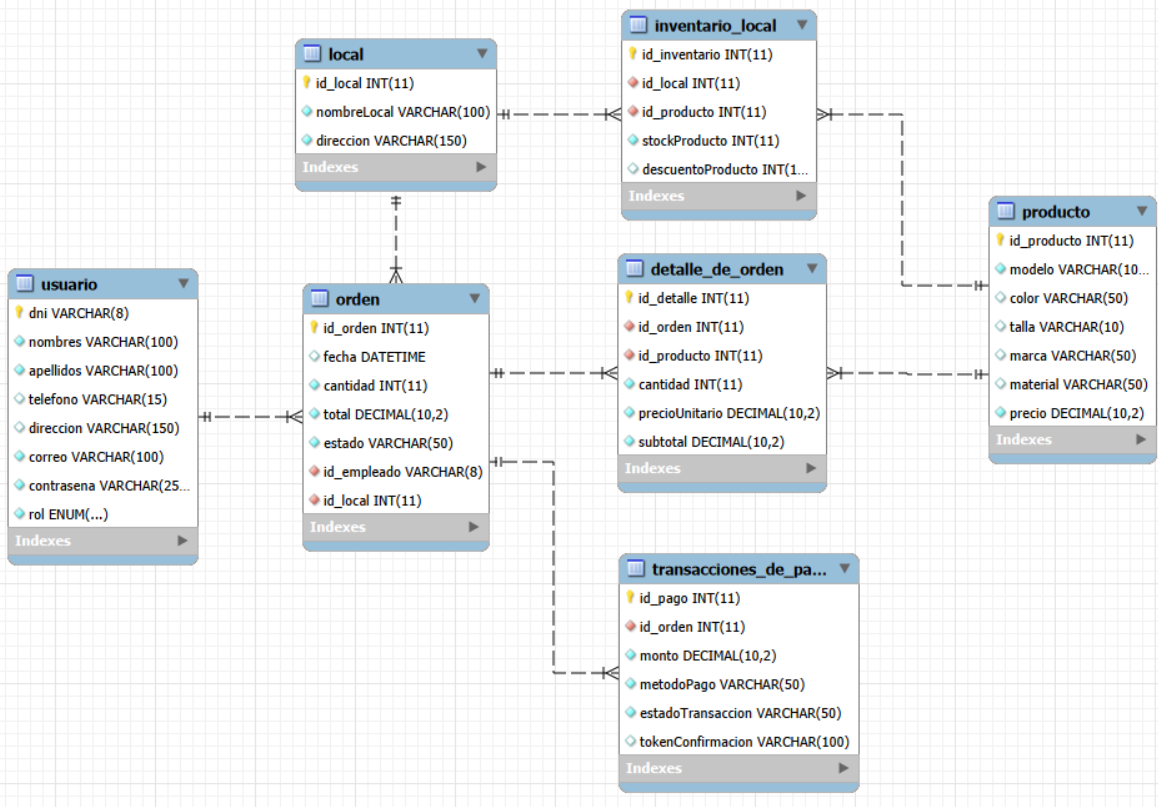
\includegraphics[width=0.92\linewidth]{figures/diagrama_bd_original.png}
\caption{Diagrama de Base de Datos y Entidades Relacionales de SYSELL.}
\label{fig:diagrama_bd}
\end{figure}

\begin{table}[H]
\centering
\small
\begin{tabularx}{\linewidth}{l>{\raggedright\arraybackslash}p{4cm}>{\raggedright\arraybackslash}X}
\toprule
\rowcolor{LightSlate}
\textbf{Tabla} & \textbf{Clave Primaria / Foráneas} & \textbf{Descripción y Campos Principales} \\
\midrule
\texttt{users} & \texttt{id} (PK), \texttt{store\_id} (FK) & Usuarios y empleados: \texttt{name}, \texttt{dni}, \texttt{phone}, \texttt{email}, \texttt{password\_hash}, \texttt{role} (\texttt{admin}/\texttt{seller}), \texttt{deleted\_at}. \\
\midrule
\texttt{stores} & \texttt{id} (PK) & Locales y almacenes: \texttt{name}, \texttt{address}, \texttt{phone}, \texttt{is\_active}, \texttt{deleted\_at}. \\
\midrule
\texttt{categories} & \texttt{id} (PK), \texttt{parent\_id} (FK) & Categorías jerárquicas: \texttt{name}, \texttt{slug}, \texttt{description}, \texttt{deleted\_at}. \\
\midrule
\texttt{products} & \texttt{id} (PK), \texttt{category\_id} (FK) & Productos padre: \texttt{name}, \texttt{brand}, \texttt{season}, \texttt{base\_price}, \texttt{base\_cost}, \texttt{image\_url}, \texttt{deleted\_at}. \\
\midrule
\texttt{product\_variants} & \texttt{id} (PK), \texttt{product\_id} (FK), \texttt{store\_id} (FK) & Variantes físicas: \texttt{sku}, \texttt{size}, \texttt{color}, \texttt{stock\_current}, \texttt{stock\_minimo}, \texttt{price\_override}. \\
\midrule
\texttt{sales} & \texttt{id} (PK), \texttt{user\_id} (FK), \texttt{store\_id} (FK), \texttt{cash\_register\_id} (FK) & Cabecera de venta: \texttt{sale\_number}, \texttt{subtotal}, \texttt{tax\_igv} (18\%), \texttt{total}, \texttt{payment\_method} (\texttt{cash}/\texttt{yape\_plin}/\texttt{transfer}), \texttt{operation\_code}, \texttt{status}, \texttt{deleted\_at}. \\
\midrule
\texttt{sale\_items} & \texttt{id} (PK), \texttt{sale\_id} (FK), \texttt{variant\_id} (FK) & Detalle de venta: \texttt{quantity}, \texttt{unit\_price}, \texttt{unit\_cost}, \texttt{subtotal}. \\
\midrule
\texttt{cash\_registers} & \texttt{id} (PK), \texttt{store\_id} (FK), \texttt{user\_id} (FK) & Sesiones de caja: \texttt{opening\_amount}, \texttt{closing\_cash\_counted}, \texttt{closing\_digital\_counted}, \texttt{expected\_amount}, \texttt{difference}, \texttt{status} (\texttt{open}/\texttt{closed}), \texttt{opened\_at}, \texttt{closed\_at}. \\
\midrule
\texttt{returns} & \texttt{id} (PK), \texttt{sale\_id} (FK), \texttt{user\_id} (FK) & Devoluciones y cambios: \texttt{returned\_variant\_id}, \texttt{new\_variant\_id}, \texttt{difference\_amount}, \texttt{reason}, \texttt{returned\_at}. \\
\midrule
\texttt{audit\_logs} & \texttt{id} (PK), \texttt{user\_id} (FK) & Bitácora de auditoría: \texttt{action}, \texttt{entity\_type}, \texttt{entity\_id}, \texttt{old\_values\_json}, \texttt{new\_values\_json}, \texttt{ip\_address}, \texttt{created\_at}. \\
\bottomrule
\end{tabularx}
\caption{Diccionario del Esquema Relacional de Base de Datos.}
\label{tab:diccionario_bd}
\end{table}

\subsection{Diagrama de Clases del Dominio}

\begin{figure}[H]
\centering
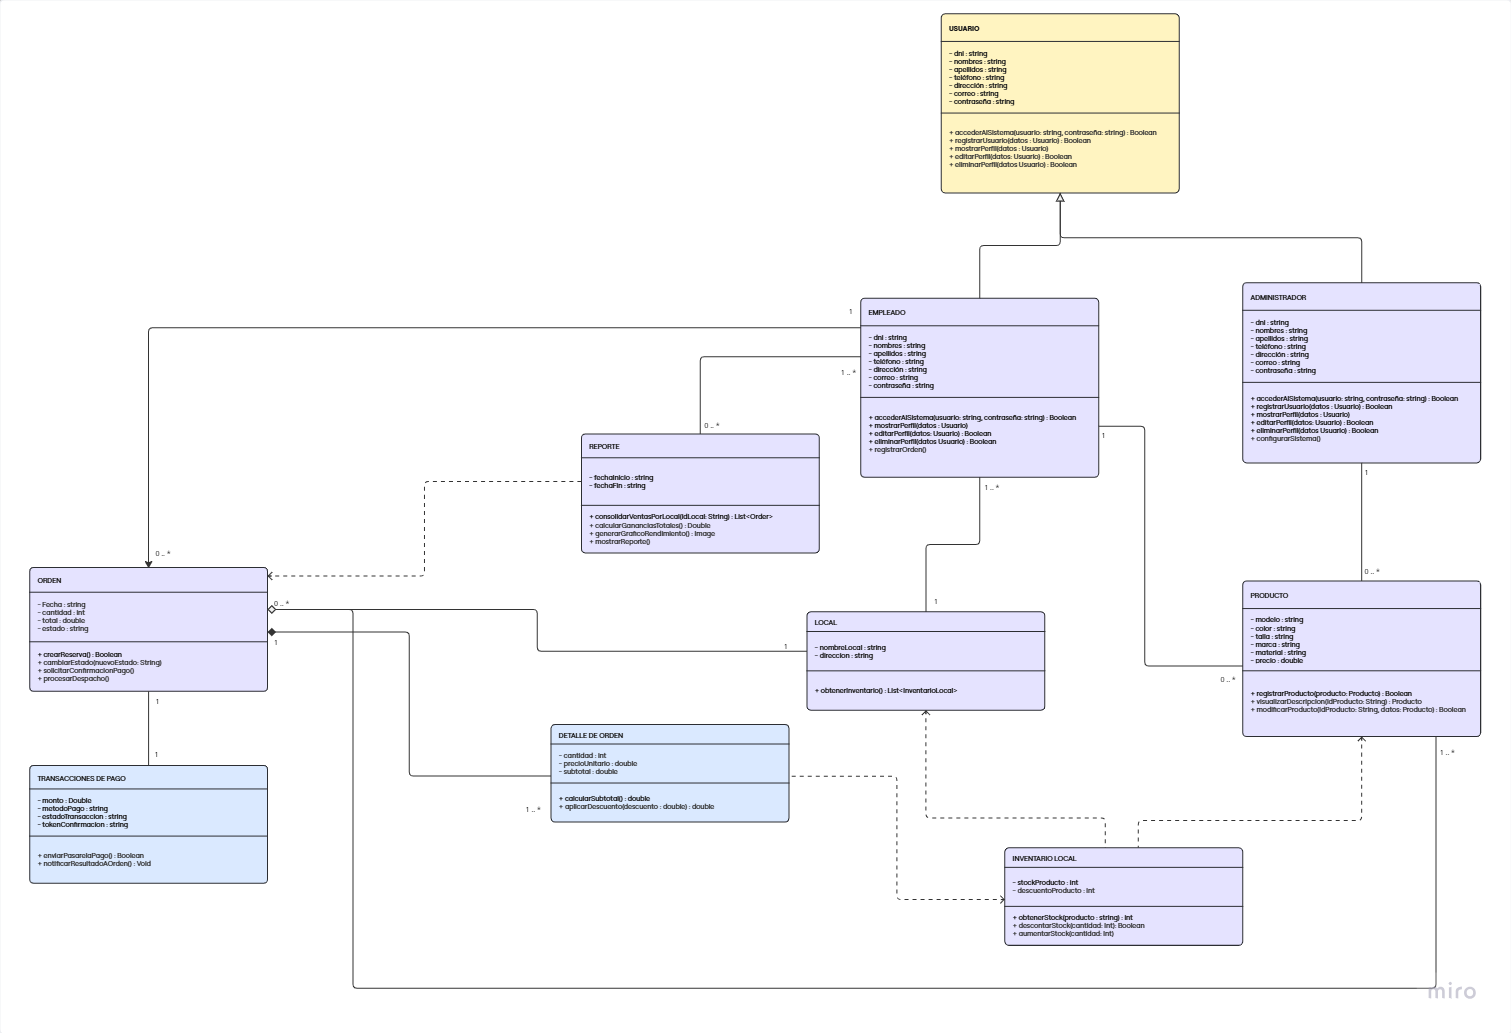
\includegraphics[width=0.88\linewidth]{figures/diagrama_clases_completo.png}
\caption{Diagrama de Clases y Relaciones de Dominio en SYSELL.}
\label{fig:diagrama_clases}
\end{figure}

\subsection{Entorno de Contenerización y DevOps (Docker \& CI/CD)}

El despliegue del sistema se encuentra completamente automatizado mediante Docker Compose:

\begin{lstlisting}[language=SQL, caption={Configuración de Servicios en \texttt{docker-compose.yml} (Extracto Estructurado)}]
version: '3.8'
services:
  sysell-frontend:
    build:
      context: ./frontend
      dockerfile: Dockerfile
    ports:
      - "80:80"
    depends_on:
      - sysell-backend

  sysell-backend:
    build:
      context: ./backend
      dockerfile: Dockerfile
    environment:
      APP_ENV: production
      DB_CONNECTION: mysql
      DB_HOST: sysell-db
      DB_DATABASE: sysell_db
      DB_USERNAME: sysell_user
      DB_PASSWORD: ${DB_PASSWORD}
    depends_on:
      - sysell-db

  sysell-db:
    image: mysql:8.0
    command: --default-authentication-plugin=mysql_native_password
    volumes:
      - mysql_data:/var/lib/mysql
    environment:
      MYSQL_DATABASE: sysell_db
      MYSQL_ROOT_PASSWORD: ${MYSQL_ROOT_PASSWORD}

volumes:
  mysql_data:
\end{lstlisting}

\newpage

% Sección 8: Diseño de Interfaces de Usuario (UI/UX)
% ==============================================================================
% SECCIÓN 8: DISEÑO DE INTERFACES DE USUARIO (DESKTOP Y RESPONSIVE 360PX)
% ==============================================================================

\section{Diseño de Interfaces de Usuario (UI/UX)}

El diseño visual del sistema web SYSELL ha sido concebido bajo un enfoque \textbf{Responsive y Mobile-First}, asegurando que todas las vistas operativas (Punto de Venta, Inventario, Reportes y Usuarios) mantengan una ergonomía y usabilidad óptimas tanto en terminales de escritorio (1920$\times$1080px) como en dispositivos móviles compactos de mostrador (\textbf{Vista Responsive 360px}).

\subsection{Módulo de Autenticación e Inicio de Sesión}

\begin{figure}[H]
\centering
\begin{subfigure}[b]{0.62\textwidth}
    \centering
    
\includegraphics[width=\textwidth]{figures/mockup_login_desktop.png}
    \caption{Vista Escritorio (Desktop --- 1920px).}
    \label{fig:login_desktop}
\end{subfigure}
\hfill
\begin{subfigure}[b]{0.32\textwidth}
    \centering
    
\includegraphics[width=\textwidth]{figures/mockup_login_mobile.png}
    \caption{Vista Responsive (360px).}
    \label{fig:login_mobile}
\end{subfigure}
\caption{Interfaz de Inicio de Sesión y Autenticación del Sistema SYSELL.}
\label{fig:mockup_login}
\end{figure}

\subsection{Módulo de Gestión y Registro de Usuarios}

\begin{figure}[H]
\centering
\begin{subfigure}[b]{0.62\textwidth}
    \centering
    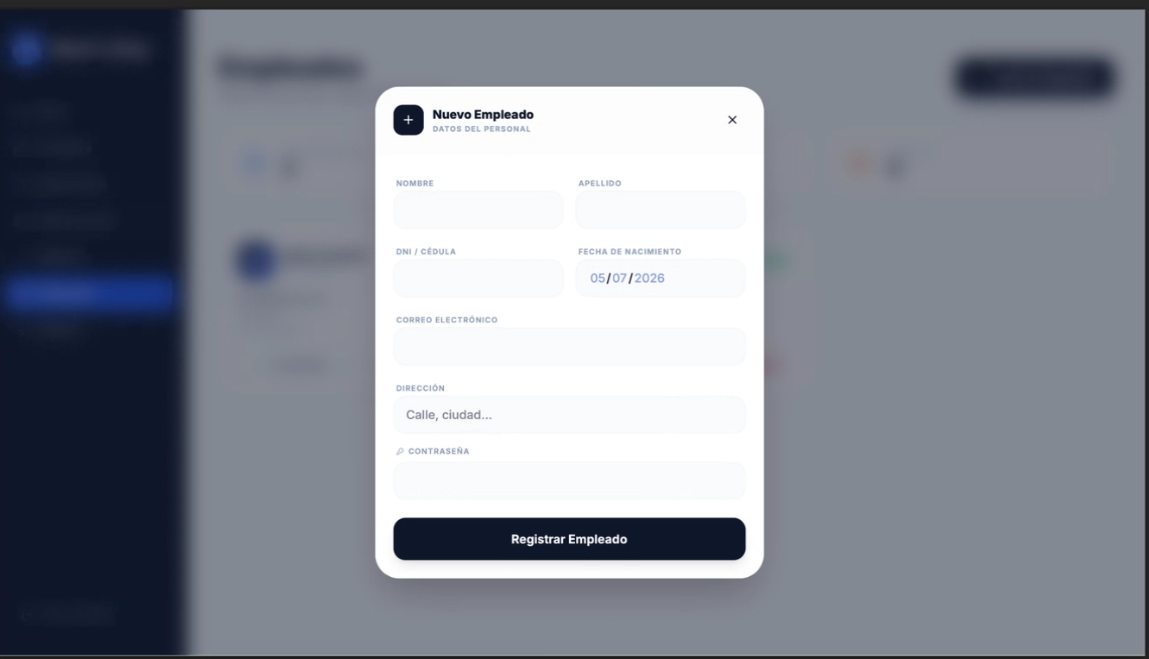
\includegraphics[width=\textwidth]{figures/mockup_usuarios_desktop.png}
    \caption{Vista Escritorio (Desktop --- 1920px).}
    \label{fig:usuarios_desktop}
\end{subfigure}
\hfill
\begin{subfigure}[b]{0.32\textwidth}
    \centering
    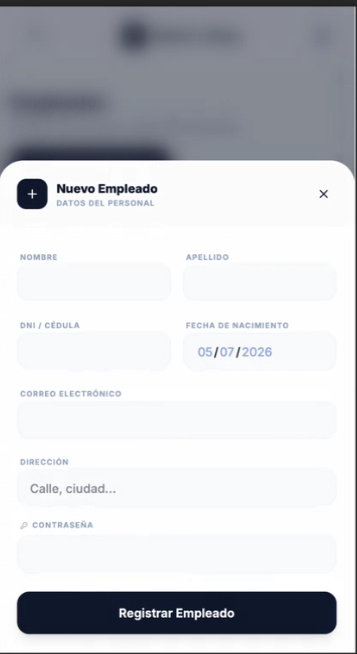
\includegraphics[width=\textwidth]{figures/mockup_usuarios_mobile.png}
    \caption{Vista Responsive (360px).}
    \label{fig:usuarios_mobile}
\end{subfigure}
\caption{Interfaz de Administración de Empleados y Control de Roles.}
\label{fig:mockup_usuarios}
\end{figure}

\subsection{Módulo de Punto de Venta (POS) y Registro de Ventas}

\begin{figure}[H]
\centering
\begin{subfigure}[b]{0.58\textwidth}
    \centering
    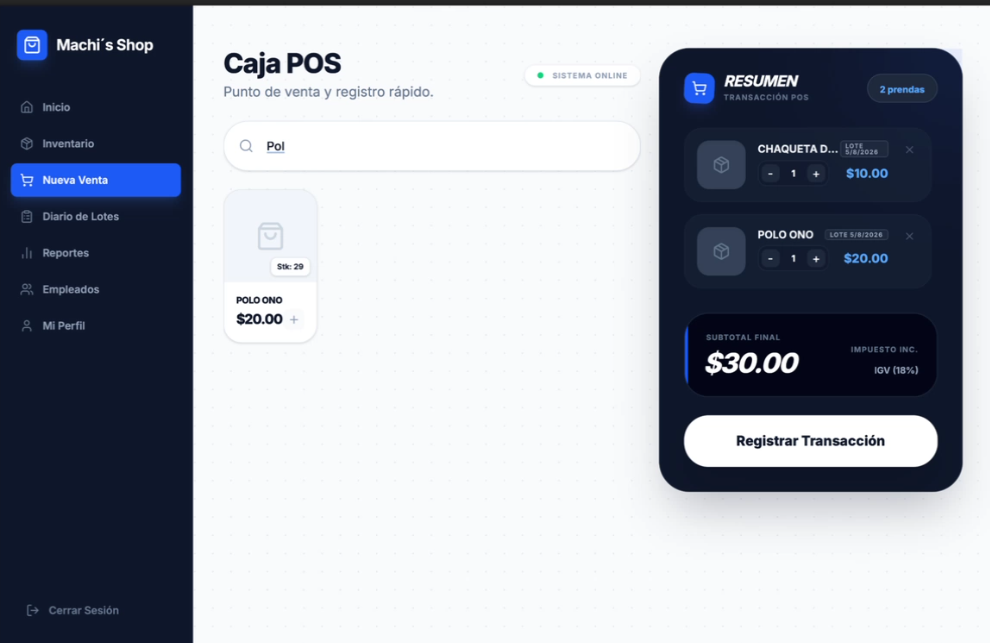
\includegraphics[width=\textwidth]{figures/mockup_ventas_desktop.png}
    \caption{Vista Escritorio (Desktop --- Punto de Venta Mostrador).}
    \label{fig:ventas_desktop}
\end{subfigure}
\hfill
\begin{subfigure}[b]{0.19\textwidth}
    \centering
    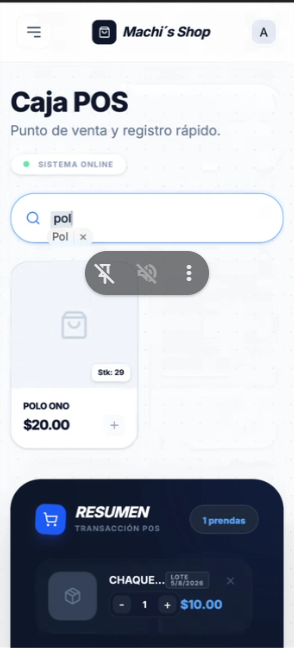
\includegraphics[width=\textwidth]{figures/mockup_ventas_mobile_1.png}
    \caption{Vista Responsive (360px) --- Catálogo.}
    \label{fig:ventas_mobile_1}
\end{subfigure}
\hfill
\begin{subfigure}[b]{0.19\textwidth}
    \centering
    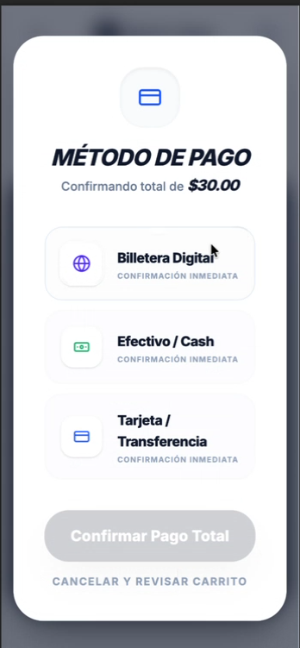
\includegraphics[width=\textwidth]{figures/mockup_ventas_mobile_2.png}
    \caption{Vista Responsive (360px) --- Carrito.}
    \label{fig:ventas_mobile_2}
\end{subfigure}
\caption{Interfaz del Módulo de Ventas y Carrito de Compras en Mostrador.}
\label{fig:mockup_ventas}
\end{figure}

\subsection{Módulo de Inventario, Catálogo y Control de Stock}

\begin{figure}[H]
\centering
\begin{subfigure}[b]{0.62\textwidth}
    \centering
    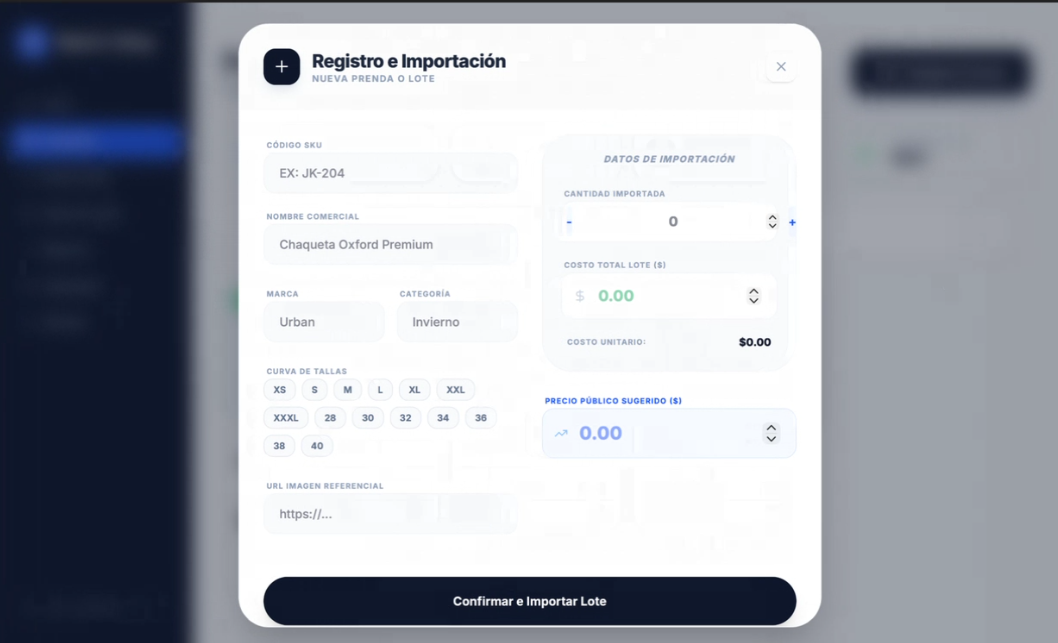
\includegraphics[width=\textwidth]{figures/mockup_inventario_desktop.png}
    \caption{Vista Escritorio (Desktop --- Tabla de Productos y Variantes).}
    \label{fig:inventario_desktop}
\end{subfigure}
\hfill
\begin{subfigure}[b]{0.32\textwidth}
    \centering
    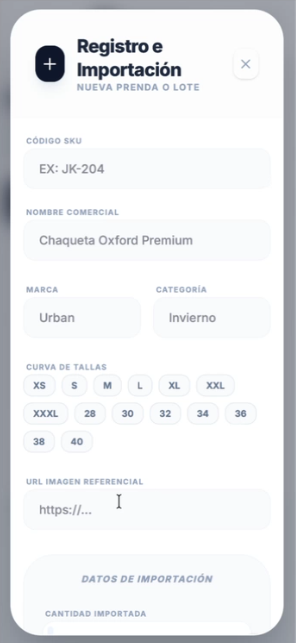
\includegraphics[width=\textwidth]{figures/mockup_inventario_mobile.png}
    \caption{Vista Responsive (360px).}
    \label{fig:inventario_mobile}
\end{subfigure}
\caption{Interfaz de Gestión de Inventario, Precios y Stock Mínimo.}
\label{fig:mockup_inventario}
\end{figure}

\subsection{Módulo de Reportes, Analítica y Balances Financieros}

\begin{figure}[H]
\centering
\begin{subfigure}[b]{0.62\textwidth}
    \centering
    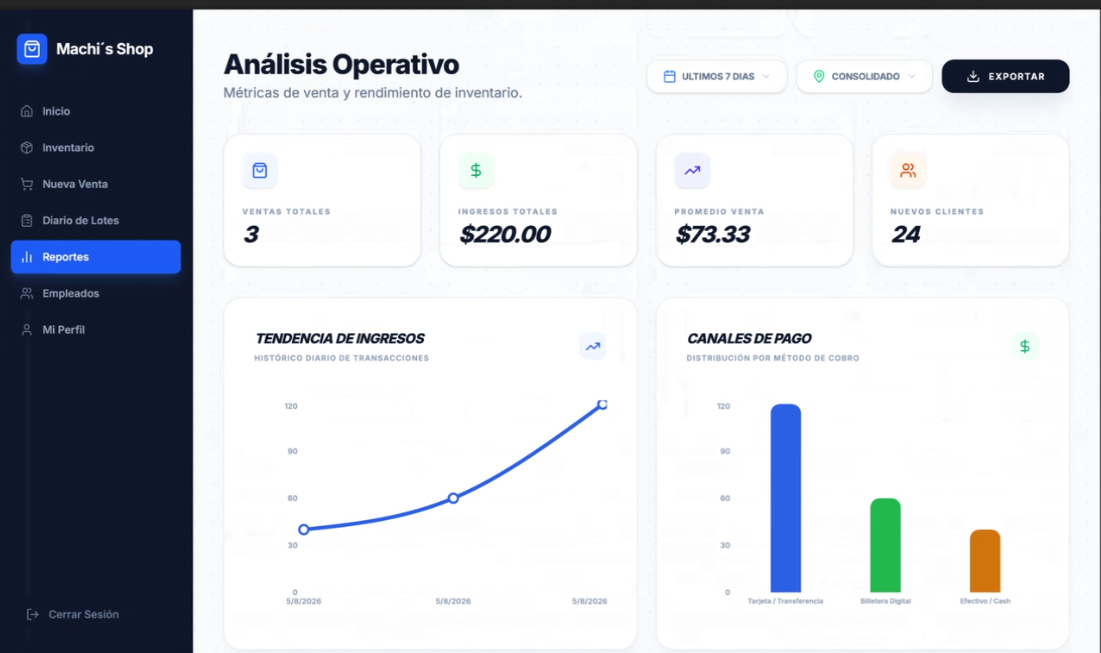
\includegraphics[width=\textwidth]{figures/mockup_reportes_desktop.png}
    \caption{Vista Escritorio (Desktop --- Gráficos y Tablas Consolidadas).}
    \label{fig:reportes_desktop}
\end{subfigure}
\hfill
\begin{subfigure}[b]{0.32\textwidth}
    \centering
    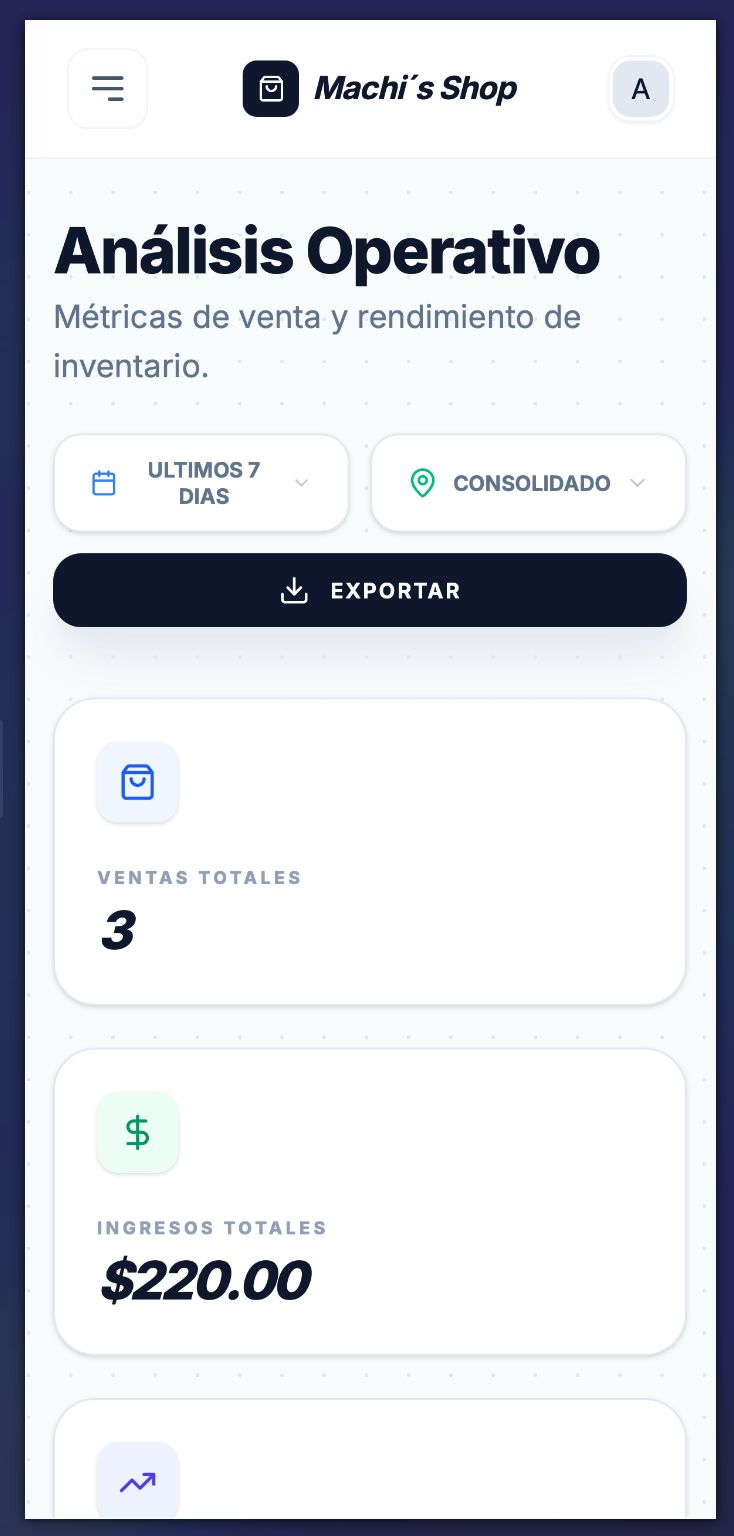
\includegraphics[width=\textwidth]{figures/mockup_reportes_mobile.png}
    \caption{Vista Responsive (360px).}
    \label{fig:reportes_mobile}
\end{subfigure}
\caption{Interfaz de Reportes Analíticos, Filtrado Temporal y Exportación.}
\label{fig:mockup_reportes}
\end{figure}

\subsection{Diagrama de Navegabilidad y Flujo de Pantallas}

\begin{figure}[H]
\centering
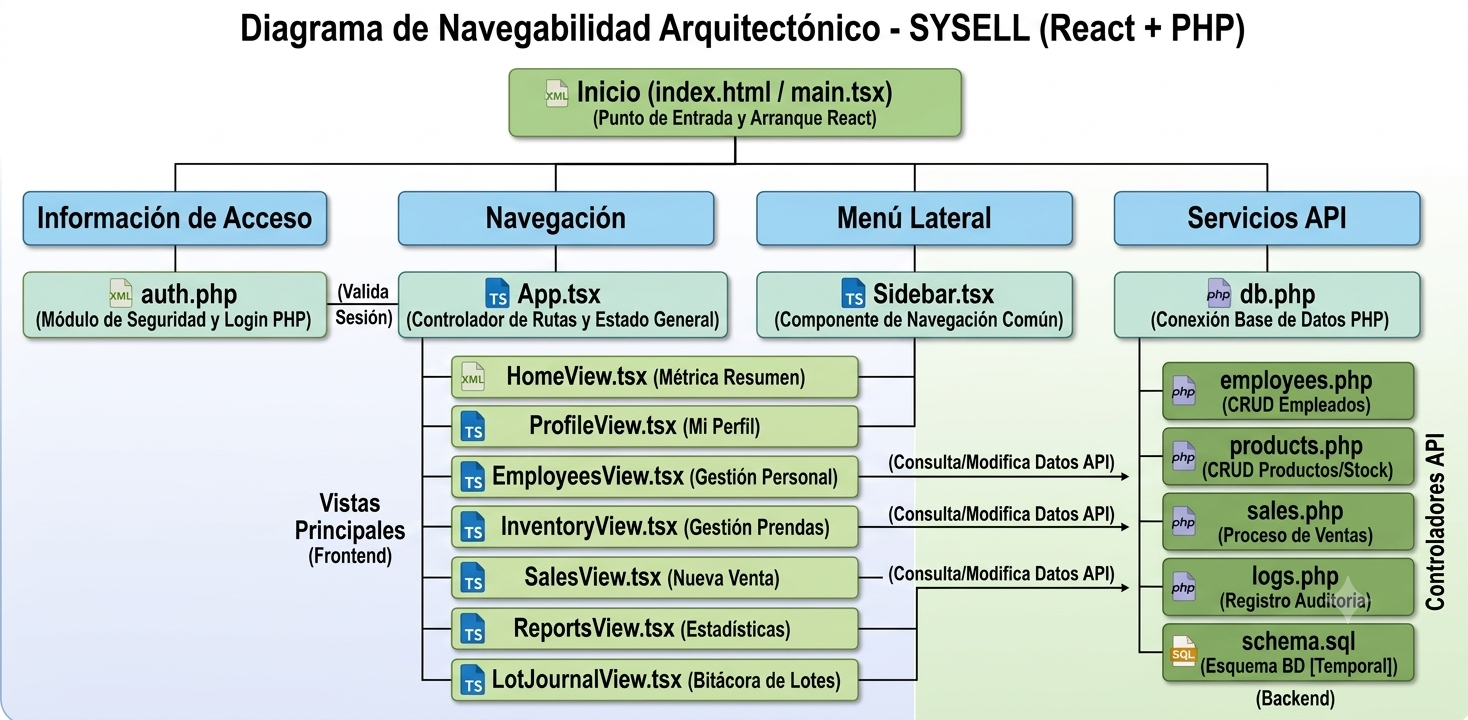
\includegraphics[width=0.85\linewidth]{figures/diagrama_navegabilidad.png}
\caption{Diagrama de Navegabilidad y Flujo de Vistas del Sistema SYSELL.}
\label{fig:diagrama_navegabilidad}
\end{figure}

\newpage

% Sección 9: Alcance Futuro y Roadmap
% ==============================================================================
% SECCIÓN 9: ALCANCE FUTURO Y ROADMAP DE EVOLUCIÓN (FASE 2 Y FASE 3)
% ==============================================================================

\section{Alcance Futuro y Roadmap de Evolución Tecnológica}

El diseño modular basado en Clean Architecture y CQRS permite proyectar una evolución continua del sistema SYSELL sin comprometer la estabilidad del núcleo transaccional. A continuación se detallan las iniciativas planificadas para las siguientes etapas de madurez digital de Comercial Machi's:

\subsection{Fase 2: Gestión de Cadena de Suministro y Facturación Electrónica SUNAT}

\begin{enumerate}[leftmargin=*]
    \item \textbf{Módulo de Compras y Cuentas por Pagar a Proveedores:}
    \begin{itemize}
        \item Registro de órdenes de compra (\textit{Purchase Orders}) y recepción formal de mercadería contra guía de remisión del proveedor.
        \item Cálculo automático del Costo Promedio Ponderado (CPP) por prenda para actualización dinámica de márgenes de ganancia.
        \item Control de deudas y cronograma de pagos a proveedores de confección textil de Lima y Tacna.
    \end{itemize}

    \item \textbf{Integración Tributaria con SUNAT (Facturación Electrónica OSE/PSE):}
    \begin{itemize}
        \item Generación automática de comprobantes de pago electrónicos en formato estándar XML UBL 2.1 (\textit{Universal Business Language}).
        \item Firma digital con certificado digital tributario y envío directo al Web Service de SUNAT / OSE.
        \item Generación de la representación impresa en PDF con código QR y Código Hash (\textit{DigestValue}), así como emisión de Boletas de Venta Electrónicas y Facturas con RUC.
    \end{itemize}
\end{enumerate}

\subsection{Fase 3: Expansión Omnicanal y E-commerce B2C}

\begin{enumerate}[leftmargin=*]
    \item \textbf{Tienda Virtual E-commerce para Clientes Finales:}
    \begin{itemize}
        \item Portal web público y optimizado para SEO donde los clientes de Comercial Machi's puedan consultar el catálogo en línea, seleccionar tallas/colores y armar su pedido.
        \item Sincronización bidireccional de stock en tiempo real entre la tienda física y la tienda virtual, evitando quiebres de inventario.
        \item Opciones de retiro en tienda física (\textit{Click \& Collect}) y despacho a domicilio en la ciudad de Tacna y envíos a nivel nacional.
    \end{itemize}

    \item \textbf{Integración de Pasarela de Pagos Web en Línea:}
    \begin{itemize}
        \item Incorporación de un checkout seguro con procesamiento de tarjetas de crédito y débito (Visa, Mastercard, American Express) mediante proveedores certificados PCI-DSS (Culqi, Niubiz o Mercado Pago).
        \item Conciliación automática de liquidaciones bancarias y comisiones de pasarela en el módulo financiero del ERP.
    \end{itemize}
\end{enumerate}

\begin{table}[H]
\centering
\small
\begin{tabularx}{\linewidth}{l>{\raggedright\arraybackslash}p{4cm}>{\raggedright\arraybackslash}Xl}
\toprule
\rowcolor{LightSlate}
\textbf{Fase} & \textbf{Módulo / Funcionalidad} & \textbf{Objetivo Estratégico y Beneficio} & \textbf{Horizonte} \\
\midrule
\textbf{Fase 1 (Actual)} & POS, Inventario, Cajas y Auditoría & Control operacional estricto de ventas físicas y arqueos. & Octubre 2026 \\
\midrule
\textbf{Fase 2} & Compras a Proveedores \& Facturación SUNAT & Automatización contable, tributaria y costeo de mercadería. & Q1 2027 \\
\midrule
\textbf{Fase 3} & E-commerce B2C \& Pasarela de Pagos Online & Expansión de ventas omnicanal y canal digital directo. & Q2 2027 \\
\bottomrule
\end{tabularx}
\caption{Roadmap de Evolución Estratégica del Sistema SYSELL.}
\label{tab:roadmap_sysell}
\end{table}

\newpage

% Sección 10: Anexos y Evidencias Académicas
% ==============================================================================
% SECCIÓN 10: ANEXOS Y EVIDENCIAS ACADÉMICAS DEL PROYECTO
% ==============================================================================

\section{Anexos y Evidencias Académicas}

En esta sección se compilan las evidencias documentales, registros de auditoría de calidad, tableros de gestión ágil en Miro, estructuración de la EDT y registros fotográficos de las visitas técnicas realizadas por el equipo a las instalaciones de Comercial Machi's.

\subsection{Anexo A: Gestión de Proyecto, EDT y Tableros Ágiles en Miro}

El proyecto fue planificado y controlado mediante la Estructura de Desglose de Trabajo (EDT) y tableros Kanban en la plataforma colaborativa Miro:

\begin{figure}[H]
\centering
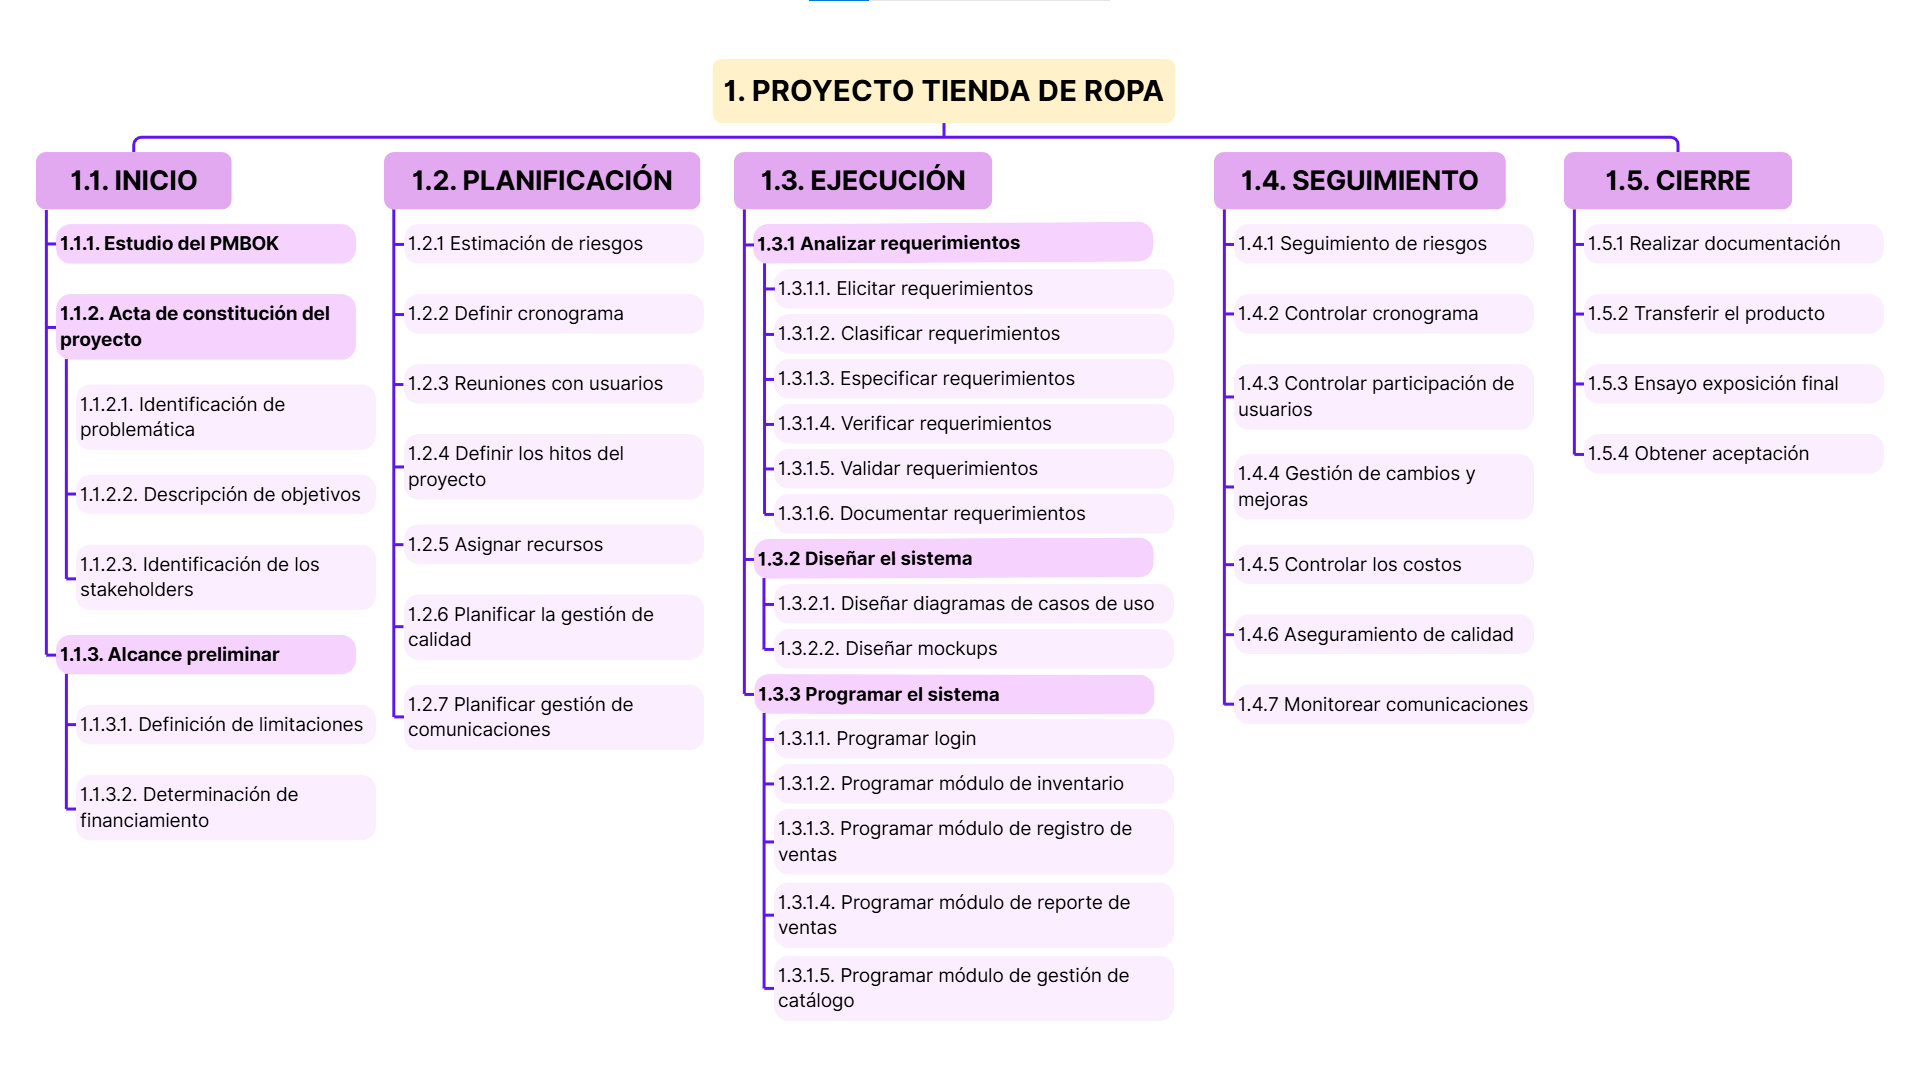
\includegraphics[width=0.92\linewidth]{figures/diagrama_edt.png}
\caption{Estructura de Desglose de Trabajo (EDT) del Proyecto SYSELL.}
\label{fig:anexo_edt}
\end{figure}

\begin{figure}[H]
\centering
\begin{subfigure}[b]{0.95\textwidth}
    \centering
    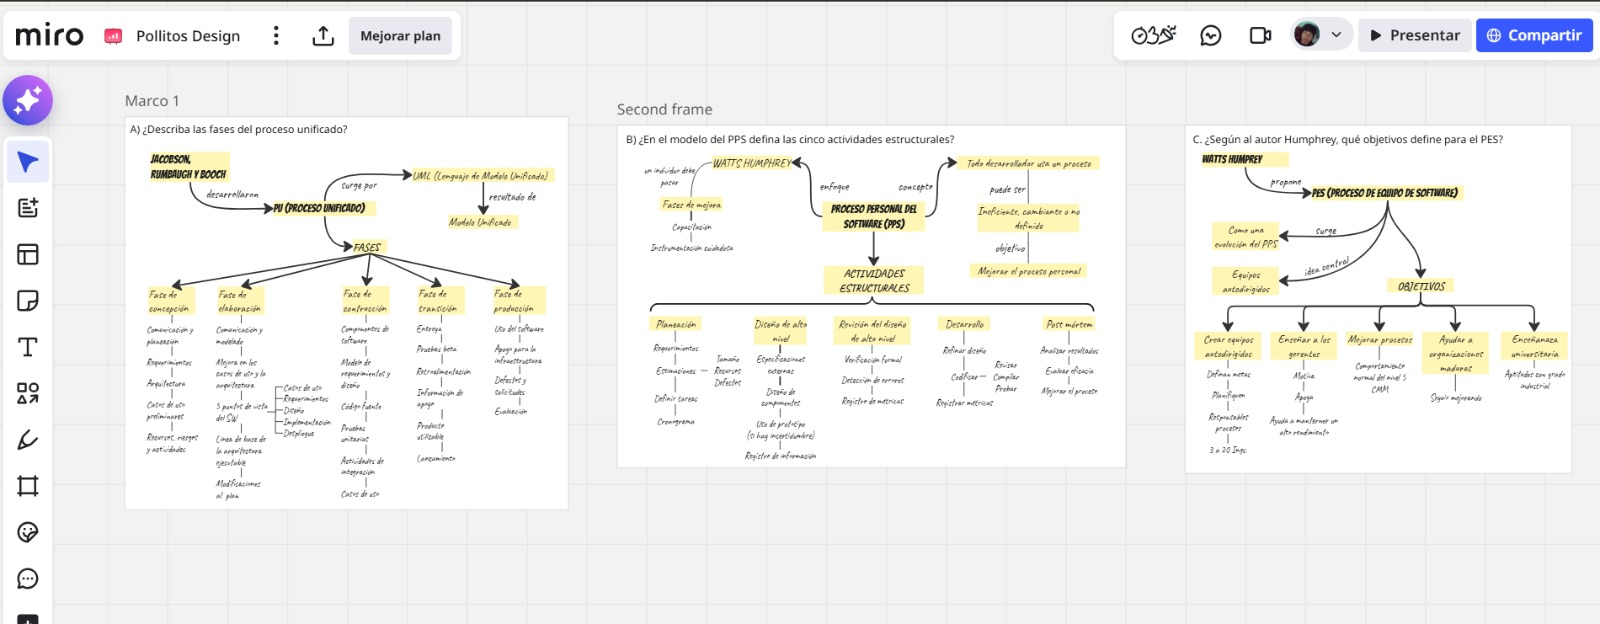
\includegraphics[width=\textwidth]{figures/miro_taskboard_1.png}
    \caption{TaskBoard en Miro --- Vista General del Backlog y Sprints de Desarrollo.}
    \label{fig:miro_1}
\end{subfigure}
\par\vspace{0.4cm}
\begin{subfigure}[b]{0.48\textwidth}
    \centering
    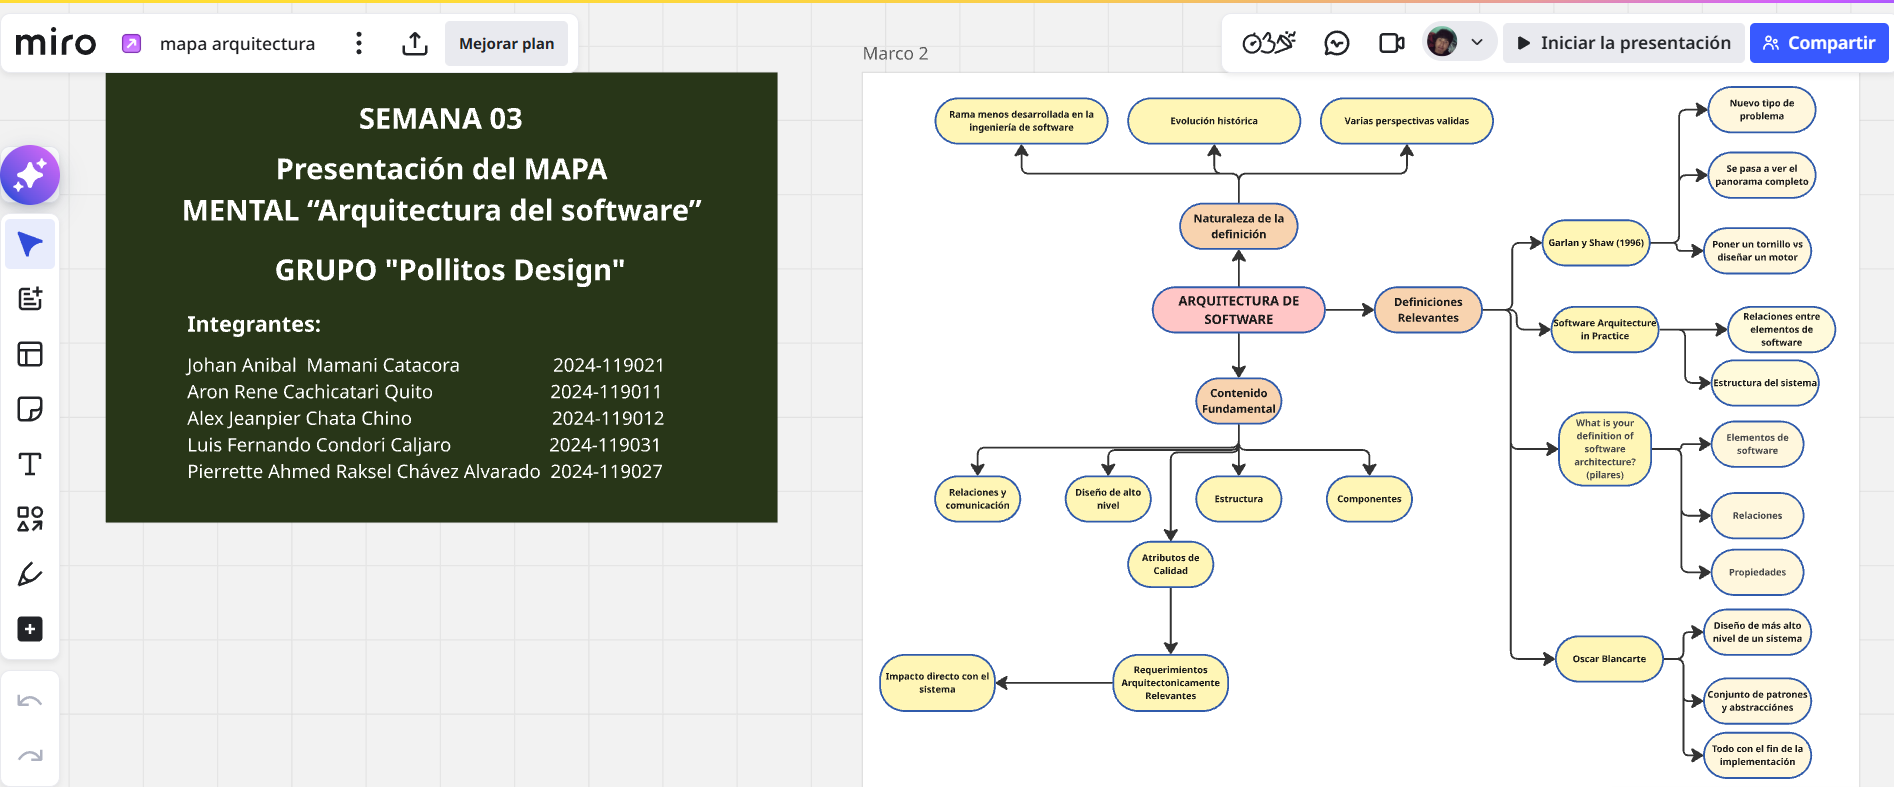
\includegraphics[width=\textwidth]{figures/miro_taskboard_2.png}
    \caption{Flujo de Tareas en Progreso y Testing.}
    \label{fig:miro_2}
\end{subfigure}
\hfill
\begin{subfigure}[b]{0.48\textwidth}
    \centering
    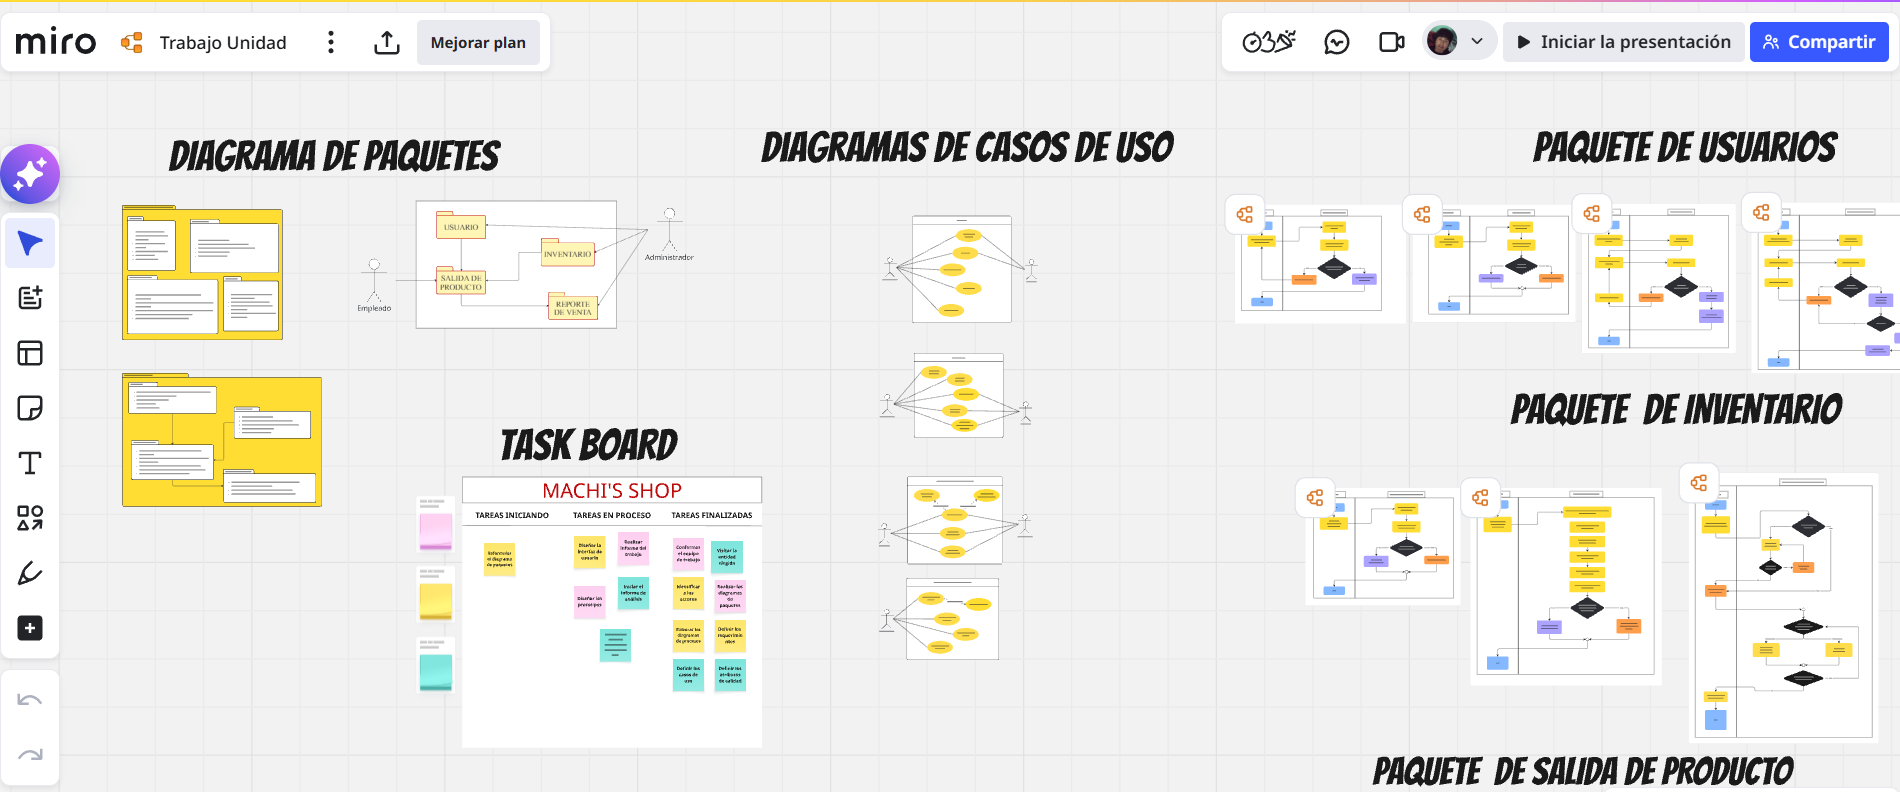
\includegraphics[width=\textwidth]{figures/miro_taskboard_3.png}
    \caption{Definición de Criterios de Aceptación (Done).}
    \label{fig:miro_3}
\end{subfigure}
\caption{Evidencias de Gestión Ágil y TaskBoard en Miro.}
\label{fig:anexo_miro}
\end{figure}

\subsection{Anexo B: Informes de Auditoría de Calidad (Interna y Externa)}

Durante el ciclo de desarrollo se llevaron a cabo evaluaciones formales de auditoría para asegurar el cumplimiento de los estándares de arquitectura y la norma ISO/IEC 25010:

\begin{figure}[H]
\centering
\begin{subfigure}[b]{0.31\textwidth}
    \centering
    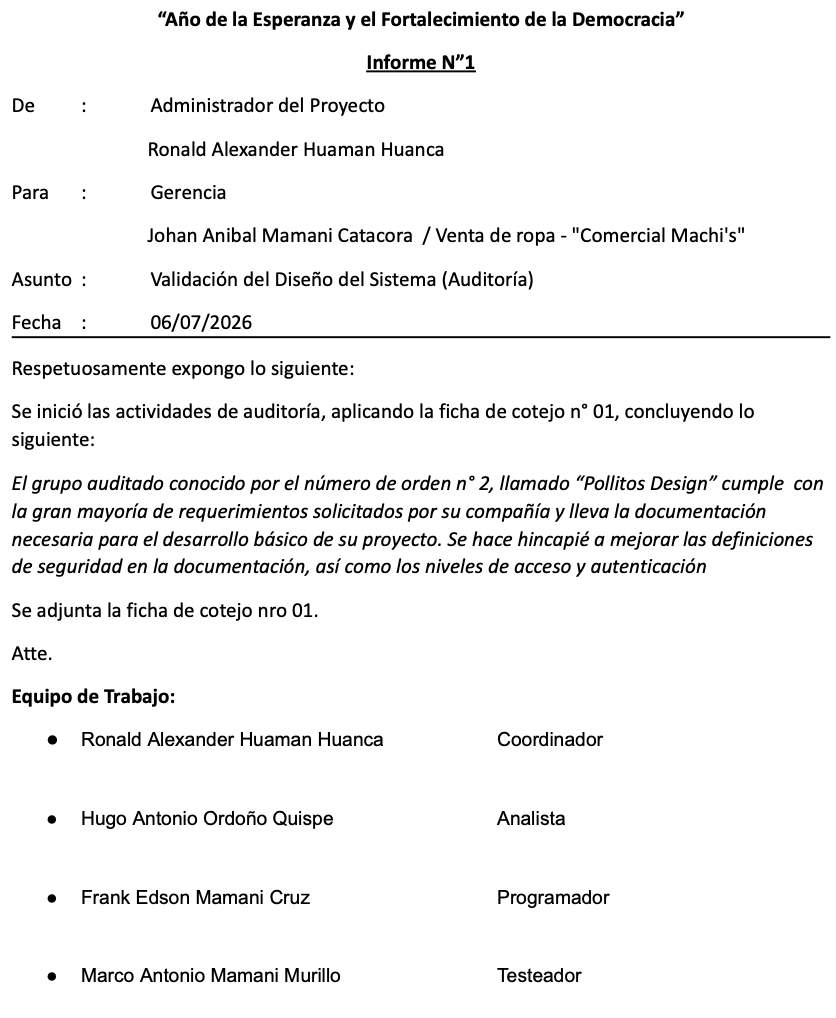
\includegraphics[width=\textwidth]{figures/auditoria_interna_p1.png}
    \caption{Auditoría Interna (Pág. 1).}
\end{subfigure}
\hfill
\begin{subfigure}[b]{0.31\textwidth}
    \centering
    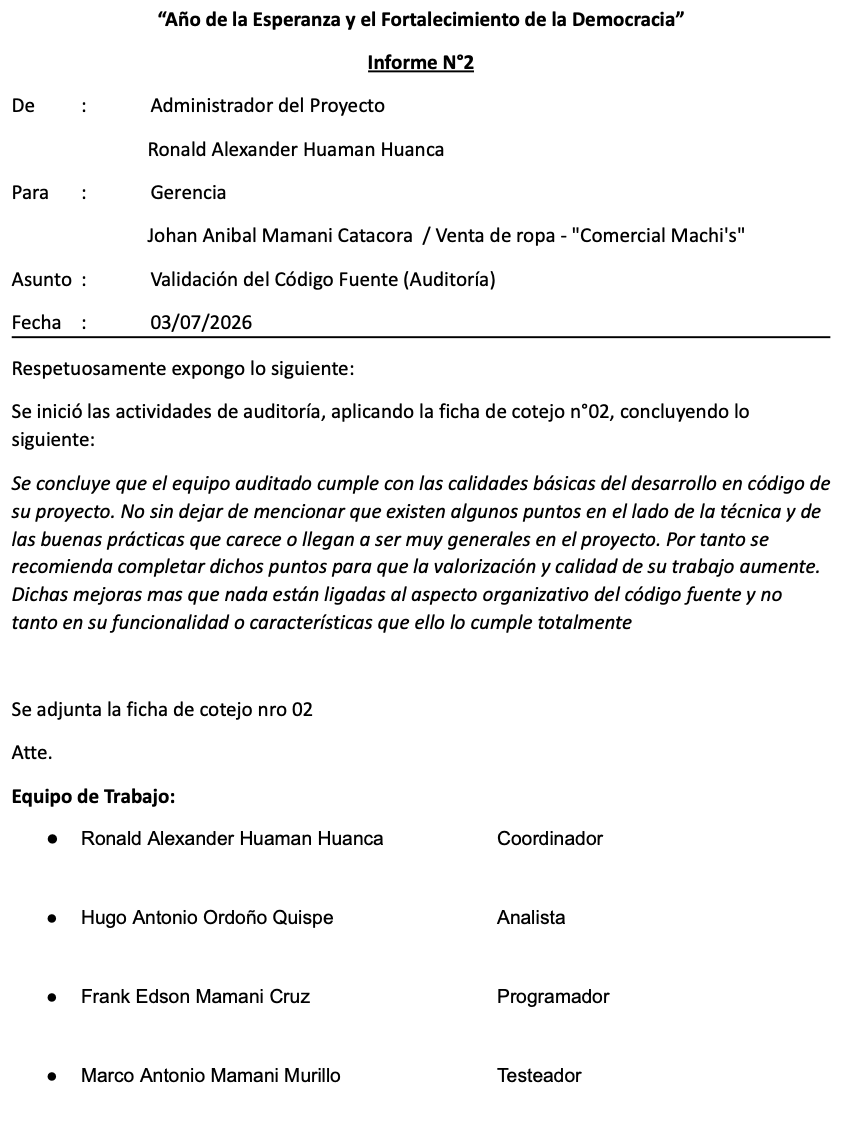
\includegraphics[width=\textwidth]{figures/auditoria_interna_p2.png}
    \caption{Auditoría Interna (Pág. 2).}
\end{subfigure}
\hfill
\begin{subfigure}[b]{0.31\textwidth}
    \centering
    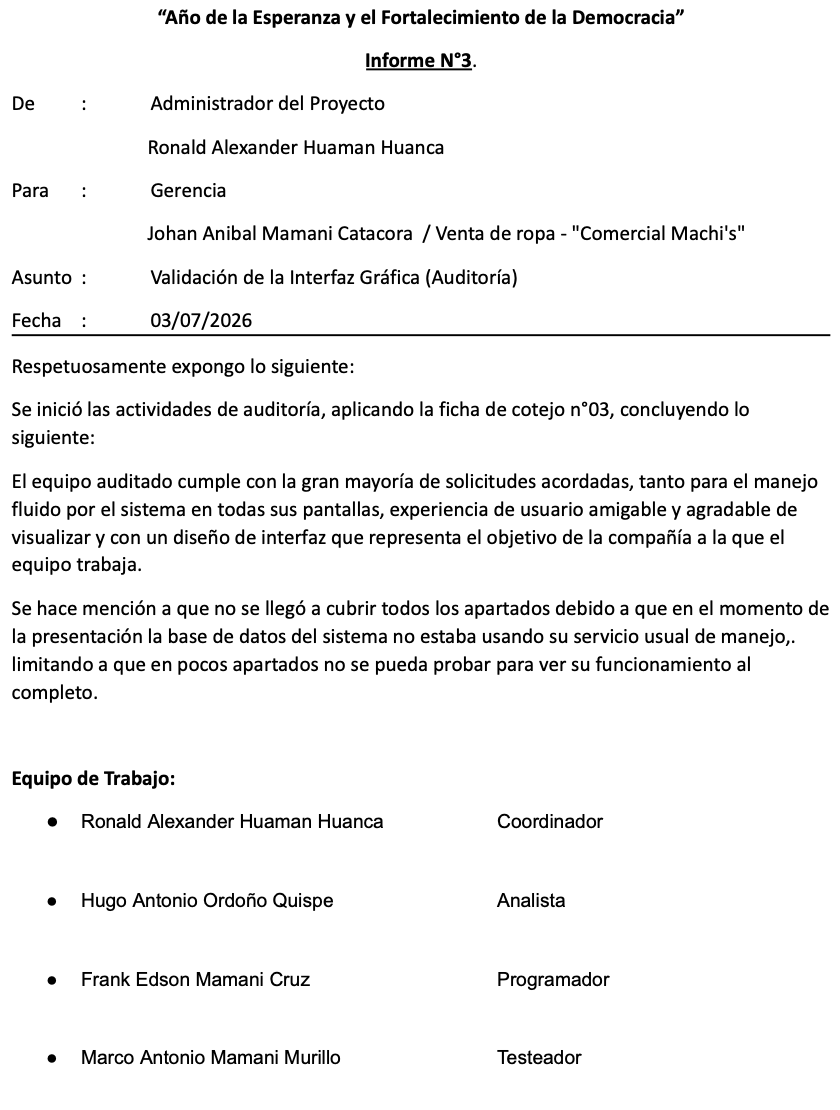
\includegraphics[width=\textwidth]{figures/auditoria_interna_p3.png}
    \caption{Auditoría Interna (Pág. 3).}
\end{subfigure}
\caption{Actas e Informes de Auditoría Interna de Software.}
\label{fig:anexo_auditoria_interna}
\end{figure}

\begin{figure}[H]
\centering
\begin{subfigure}[b]{0.48\textwidth}
    \centering
    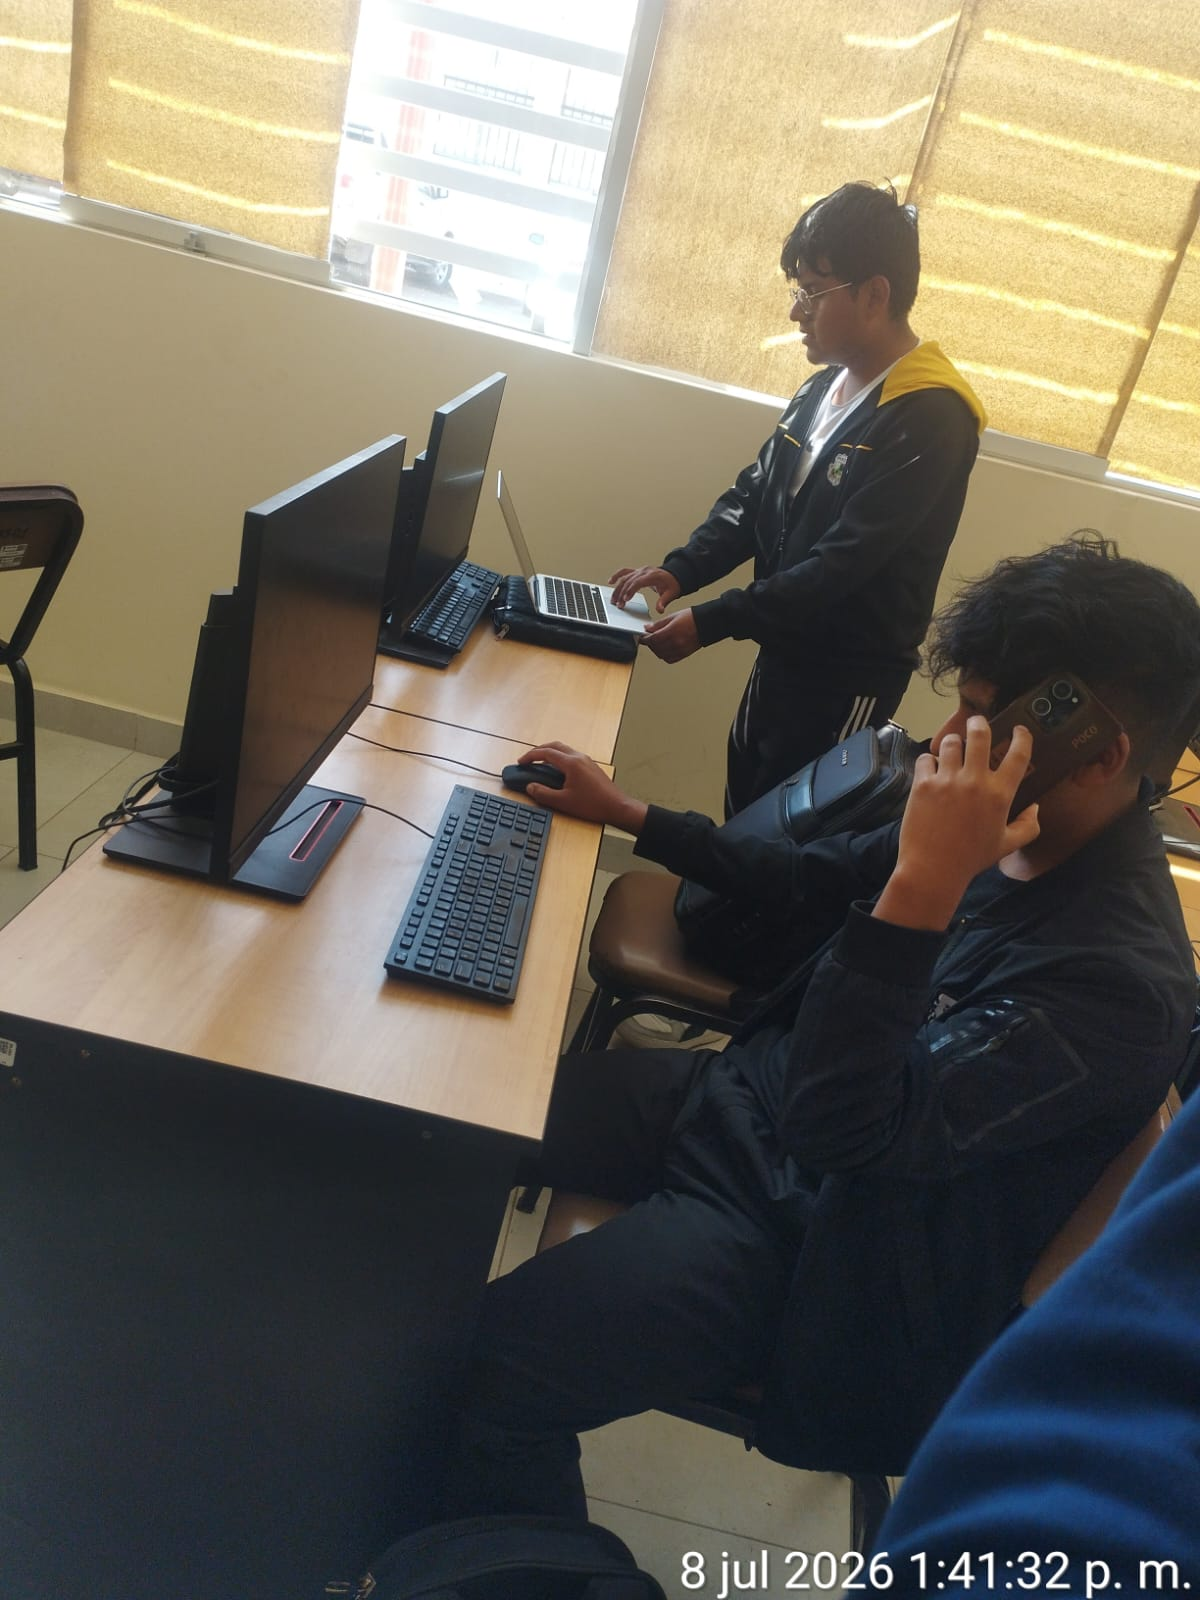
\includegraphics[width=\textwidth]{figures/auditoria_externa_p1.png}
    \caption{Informe de Auditoría Externa N° 3 --- Hallazgos.}
\end{subfigure}
\hfill
\begin{subfigure}[b]{0.48\textwidth}
    \centering
    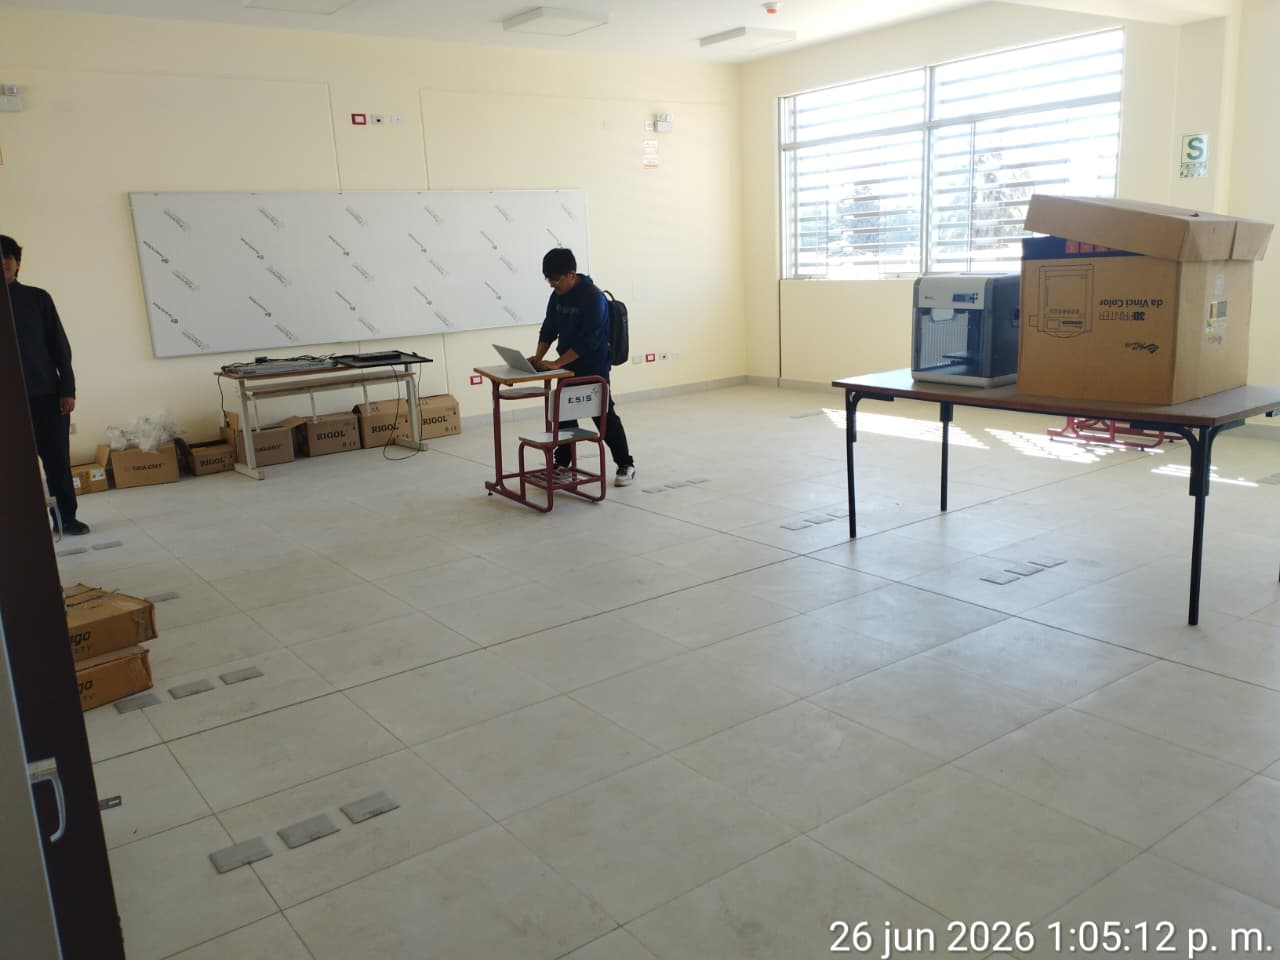
\includegraphics[width=\textwidth]{figures/auditoria_externa_p2.png}
    \caption{Conclusiones y Acciones Correctivas de Auditoría Externa.}
\end{subfigure}
\caption{Dictámenes de Auditoría Externa del Sistema SYSELL.}
\label{fig:anexo_auditoria_externa}
\end{figure}

\subsection{Anexo C: Evidencias de Trabajo de Campo y Equipo}

\begin{figure}[H]
\centering
\begin{subfigure}[b]{0.48\textwidth}
    \centering
    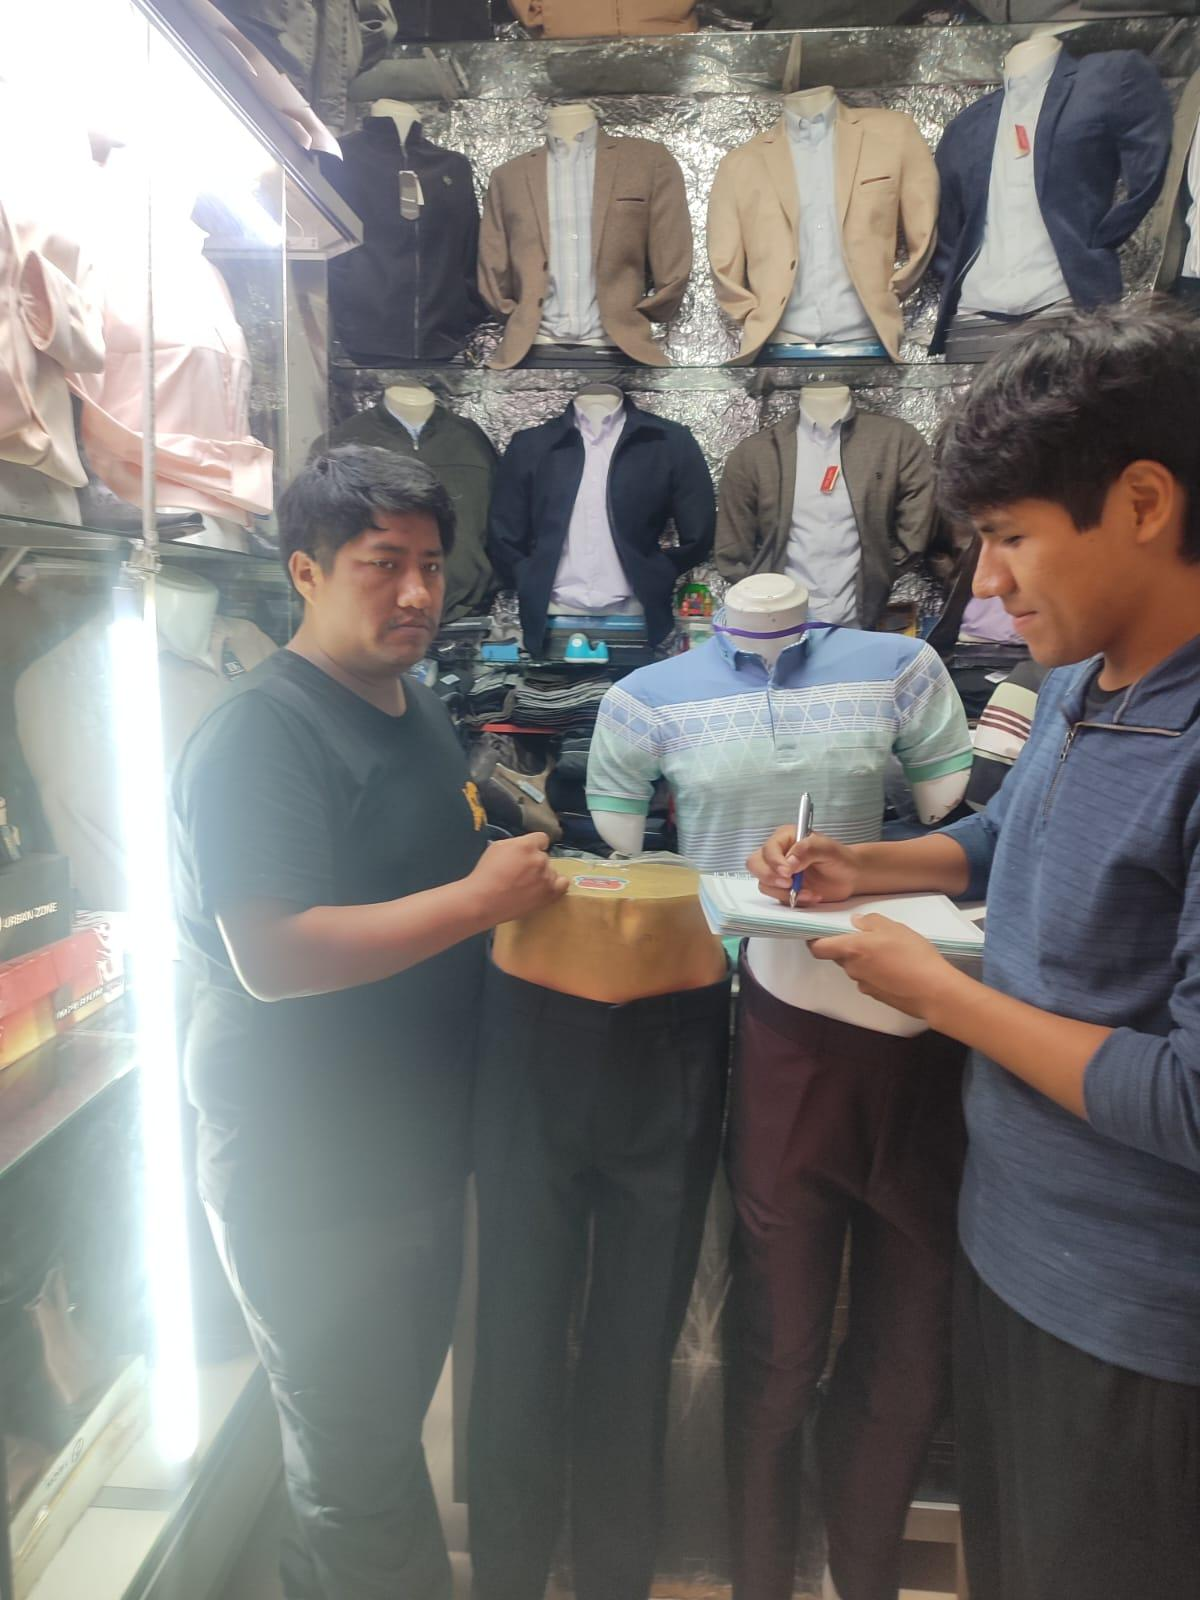
\includegraphics[width=\textwidth]{figures/evidencia_visita_tienda.jpg}
    \caption{Visita Técnica a Comercial Machi's (Levantamiento de Información).}
    \label{fig:visita_tienda}
\end{subfigure}
\hfill
\begin{subfigure}[b]{0.48\textwidth}
    \centering
    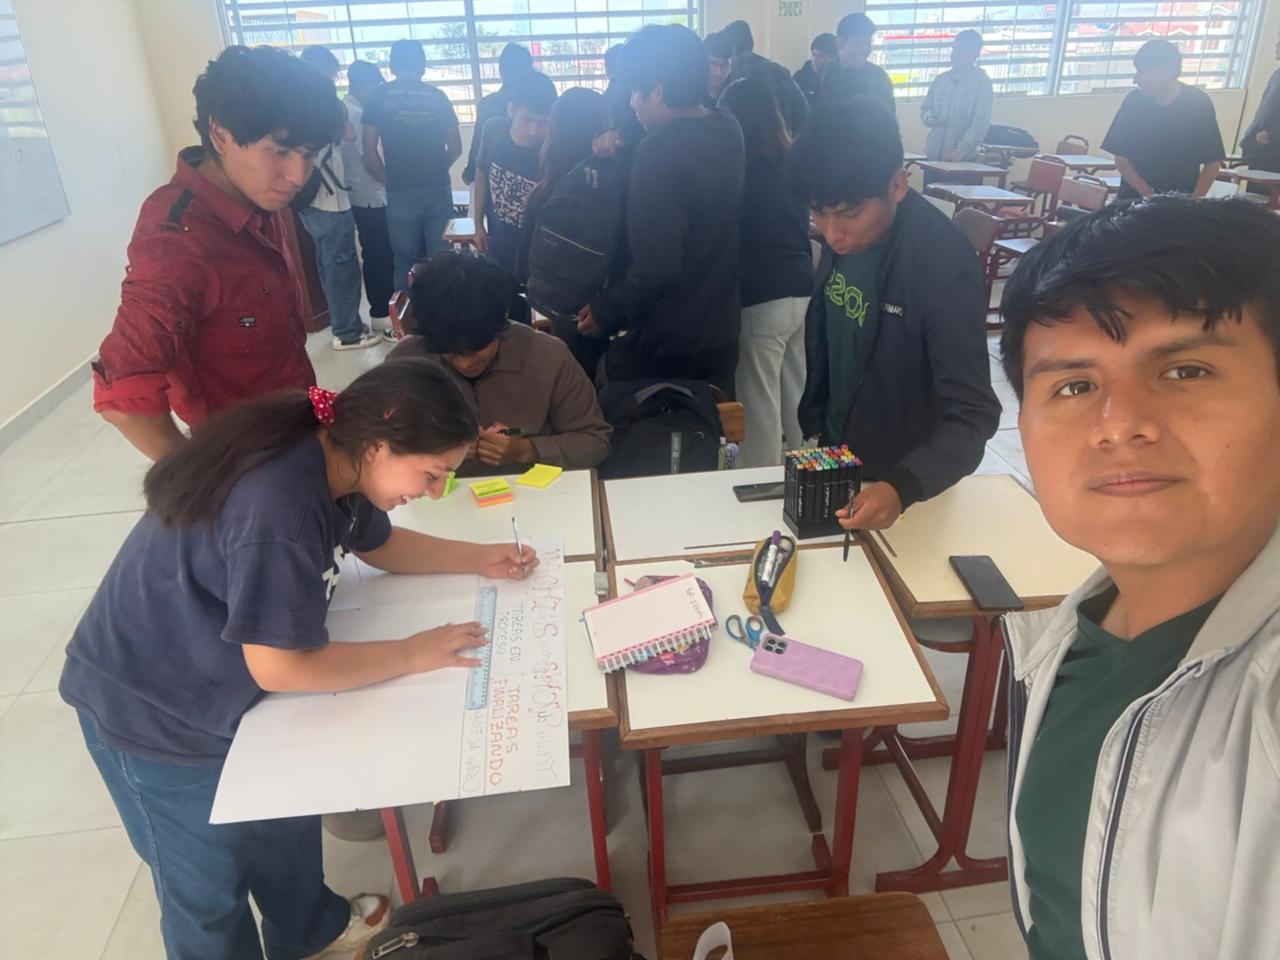
\includegraphics[width=\textwidth]{figures/evidencia_equipo_1.png}
    \caption{Sesión de Trabajo y Modelado de Arquitectura.}
    \label{fig:equipo_1}
\end{subfigure}
\par\vspace{0.4cm}
\begin{subfigure}[b]{0.48\textwidth}
    \centering
    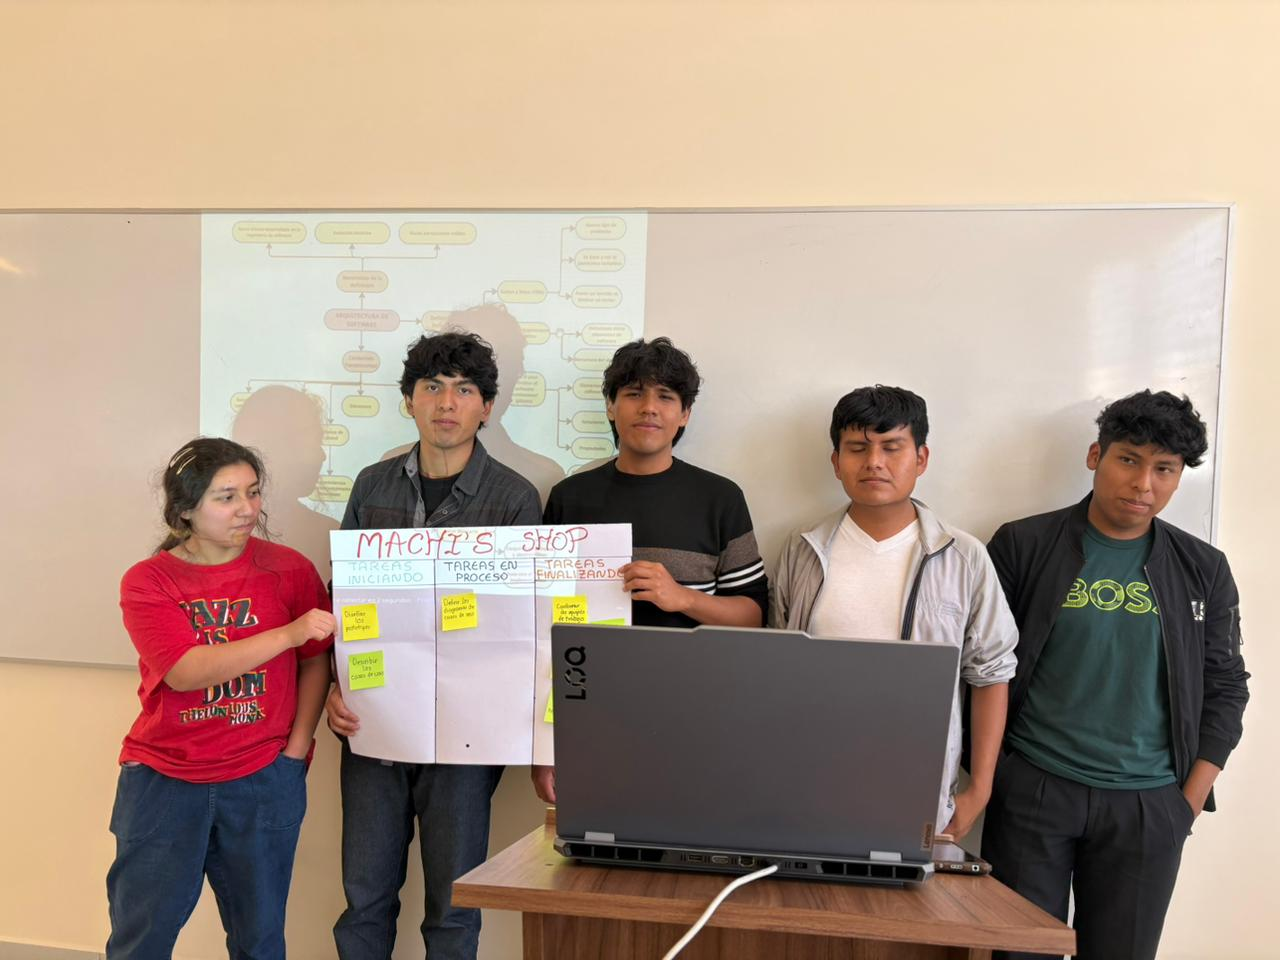
\includegraphics[width=\textwidth]{figures/evidencia_equipo_2.png}
    \caption{Revisión de Casos de Uso y Base de Datos.}
    \label{fig:equipo_2}
\end{subfigure}
\hfill
\begin{subfigure}[b]{0.48\textwidth}
    \centering
    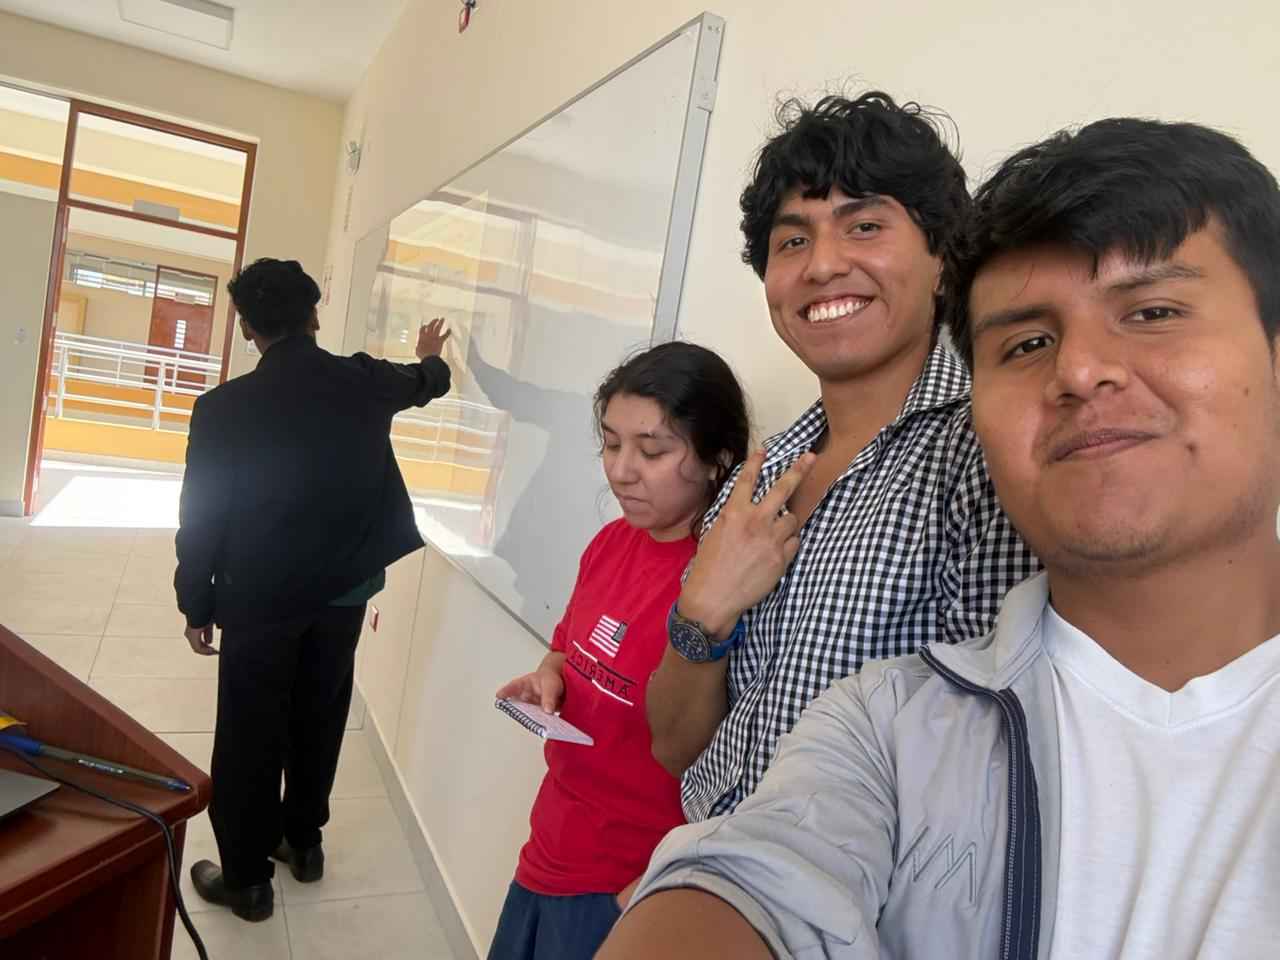
\includegraphics[width=\textwidth]{figures/evidencia_equipo_3.png}
    \caption{Sesión de Validación y Pruebas con el Asesor.}
    \label{fig:equipo_3}
\end{subfigure}
\caption{Evidencias Fotográficas del Equipo de Desarrollo y Visitas Técnicas.}
\label{fig:anexo_fotos_equipo}
\end{figure}

\subsection{Anexo D: Matriz de Trazabilidad de Requisitos (RTM)}

A continuación se resume la matriz de trazabilidad entre Requerimientos Funcionales, Reglas de Negocio, Historias de Usuario y Métodos de la API REST del backend:

\begin{table}[H]
\centering
\scriptsize
\begin{tabularx}{\linewidth}{l>{\raggedright\arraybackslash}Xll>{\raggedright\arraybackslash}p{4.5cm}}
\toprule
\rowcolor{LightSlate}
\textbf{Req.} & \textbf{Descripción Resumida} & \textbf{Regla} & \textbf{HU} & \textbf{Endpoint API REST Backend} \\
\midrule
\textbf{R-01} & Registro de Empleados & RN-08 & HU-01 & \texttt{POST /api/v1/users} \\
\textbf{R-02} & Login y Autenticación Sanctum & RN-08 & HU-01 & \texttt{POST /api/v1/auth/login} \\
\textbf{R-04} & Baja Lógica Empleado (Soft Delete) & RN-04 & HU-07 & \texttt{DELETE /api/v1/users/\{id\}} \\
\textbf{R-06} & Salida y Descuento Atómico de Stock & RN-02 & HU-03 & \texttt{POST /api/v1/sales} \\
\textbf{R-07} & Registro de Ganancias y Margen & RN-01 & HU-03 & \texttt{GET /api/v1/metrics/profit} \\
\textbf{R-08} & Registro de Venta POS en Mostrador & RN-01 & HU-03 & \texttt{POST /api/v1/sales} \\
\textbf{R-09} & Búsqueda Rápida de Productos & RN-10 & HU-03 & \texttt{GET /api/v1/products/search} \\
\textbf{R-10} & Restricción de Ingresos a Admin & RN-09 & HU-01 & \texttt{GET /api/v1/finances} \\
\textbf{R-12} & Alerta de Stock Mínimo & RN-03 & HU-04 & \texttt{GET /api/v1/inventory/alerts} \\
\textbf{R-14} & Baja Lógica Producto (Soft Delete) & RN-04 & HU-07 & \texttt{DELETE /api/v1/products/\{id\}} \\
\textbf{R-18} & Exportación Reportes PDF/Excel & RN-01 & HU-06 & \texttt{GET /api/v1/reports/export} \\
\textbf{R-19} & Devoluciones y Cambios & RN-06 & HU-05 & \texttt{POST /api/v1/returns} \\
\textbf{R-20} & Gestión de Múltiples Locales & RN-02 & HU-06 & \texttt{POST /api/v1/stores} \\
\textbf{R-23} & Cierre Diario de Caja y Arqueo & RN-07 & HU-06 & \texttt{POST /api/v1/cash/close} \\
\textbf{R-24} & Recuperación de Contraseña & RN-08 & HU-01 & \texttt{POST /api/v1/auth/forgot-password} \\
\textbf{R-25} & Bloqueo y Cierre Inactividad & RN-08 & HU-02 & \textit{Middleware / Sanctum} \\
\textbf{R-26} & Logs de Auditoría del Sistema & RN-09 & HU-07 & \texttt{GET /api/v1/audit-logs} \\
\textbf{R-27} & Filtros Multicriterio (Talla/Color) & RN-10 & HU-03 & \texttt{GET /api/v1/products/filter} \\
\textbf{R-28} & Dashboard Ejecutivo Tiempo Real & RN-01 & HU-01 & \texttt{GET /api/v1/dashboard/kpis} \\
\bottomrule
\end{tabularx}
\caption{Matriz de Trazabilidad de Requisitos (RTM) del Sistema SYSELL.}
\label{tab:matriz_trazabilidad}
\end{table}


\end{document}
